\documentclass[a4paper,twoside]{article}
\usepackage[T1]{fontenc}
\usepackage[bahasa]{babel}
\usepackage{graphicx}
\usepackage{graphics}
\usepackage{float}
\usepackage[cm]{fullpage}
\pagestyle{myheadings}
\usepackage{etoolbox}
\usepackage{setspace} 
\usepackage{lipsum} 
\setlength{\headsep}{30pt}
\usepackage[inner=2cm,outer=2.5cm,top=2.5cm,bottom=2cm]{geometry} %margin
\usepackage{multirow}
% \pagestyle{empty}

\makeatletter
\renewcommand{\@maketitle} {\begin{center} {\LARGE \textbf{ \textsc{\@title}} \par} \bigskip {\large \textbf{\textsc{\@author}} }\end{center} }
\renewcommand{\thispagestyle}[1]{}
\markright{\textbf{\textsc{Laporan Perkembangan Pengerjaan Skripsi\textemdash Sem. Genap 2015/2016}}}

\onehalfspacing

\graphicspath{{./Gambar/}}% folder tempat gambar 
 
\begin{document}

\title{\@judultopik}
\author{\nama \textendash \@npm} 

%ISILAH DATA BERIKUT INI:
\newcommand{\nama}{Andrianto Sugiarto}
\newcommand{\@npm}{2013730046}
\newcommand{\tanggal}{05/05/2018} %Tanggal pembuatan dokumen
\newcommand{\@judultopik}{Migrasi SIAModels dan IFStudentPortal ke Kurikulum 2018} % Judul/topik anda
\newcommand{\kodetopik}{PAN4402}
\newcommand{\jumpemb}{1} % Jumlah pembimbing, 1 atau 2
\newcommand{\pembA}{Pascal Alfadian}
\newcommand{\pembB}{-}
\newcommand{\semesterPertama}{44 - Genap 17/18} % semester pertama kali topik diambil, angka 1 dimulai dari sem Ganjil 96/97
\newcommand{\lamaSkripsi}{1} % Jumlah semester untuk mengerjakan skripsi s.d. dokumen ini dibuat
\newcommand{\kulPertama}{Skripsi 1} % Kuliah dimana topik ini diambil pertama kali
\newcommand{\tipePR}{B} % tipe progress report :
% A : dokumen pendukung untuk pengambilan ke-2 di Skripsi 1
% B : dokumen untuk reviewer pada presentasi dan review Skripsi 1
% C : dokumen pendukung untuk pengambilan ke-2 di Skripsi 2

% Dokumen hasil template ini harus dicetak bolak-balik !!!!

\maketitle

\pagenumbering{arabic}

\section{Data Skripsi} %TIDAK PERLU MENGUBAH BAGIAN INI !!!
Pembimbing utama/tunggal: {\bf \pembA}\\
Pembimbing pendamping: {\bf \pembB}\\
Kode Topik : {\bf \kodetopik}\\
Topik ini sudah dikerjakan selama : {\bf \lamaSkripsi} semester\\
Pengambilan pertama kali topik ini pada : Semester {\bf \semesterPertama} \\
Pengambilan pertama kali topik ini di kuliah : {\bf \kulPertama} \\
Tipe Laporan : {\bf \tipePR} -
\ifdefstring{\tipePR}{A}{
			Dokumen pendukung untuk {\BF pengambilan ke-2 di Skripsi 1} }
		{
		\ifdefstring{\tipePR}{B} {
				Dokumen untuk reviewer pada presentasi dan {\bf review Skripsi 1}}
			{	Dokumen pendukung untuk {\bf pengambilan ke-2 di Skripsi 2}}
		}
		
\section{Latar Belakang}

\paragraph{} IFStudentPortal merupakan sistem informasi berbasis  \textit{web} yang dibuat menggunakan Play Framework untuk Teknik Informatika UNPAR. Selain itu, data-data yang terdapat pada IFStudentPortal diolah dari Portal Akademik Mahasiswa dengan ekstraksi data dari situs web menggunakan \textit{library} jsoup. IFStudentPortal merupakan aplikasi buatan Herfan Heryandi dan kontributor lainnya. Fitur-fitur dari IFStudentPortal yaitu memeriksa prasyarat mata kuliah, memeriksa syarat yang masih kurang untuk kelulusan dan melihat jadwal kuliah. Catatan akademik dari fitur-fitur pada IFStudentPortal diambil berdasarkan catatan akademik mahasiswa yang login (terpersonalisasi).

Pada saat ini Program Studi Informatika dalam proses perubahan kurikulum dari 2013 ke 2018. Pada draft kurikulum 2018 versi 0.8 sudah memperlihatkan beberapa perbedaan seperti dalam kode mata kuliah (contoh: AIF401 menjadi AIF184001), struktur kuliah serta prasyaratnya, konversi dari mata kuliah kurikulum 2013, Nilai Akhir lebih bervariasi (ada A, A-, B+, dst), perbedaan dalam syarat kelulusan (tidak ada lagi pilihan wajib), dll. Dari perbedaan-perbedaan tersebut dapat dilihat bahwa diperlukan perubahan terhadap IFStudentPortal yang saat ini mendukung kurikulum 2013. Perbedaan syarat kelulusan pada kurikulum 2018 dengan kurikulum 2013 membuat diperlukan beberapa penyesuaian dengan aturan kelulusan untuk angkatan yang sudah mengambil mata kuliah pada kurikulum 2013.

Pada SIAModels merupakan kelas-kelas dalam bahasa Java yang merepresentasikan Sistem Informasi Akademik Teknik Informatika UNPAR. Untuk mendukung perubahan kurikulum dari 2013 ke 2018 yang dilakukan oleh Program Studi Informatika, perlu dilakukan konversi terhadap IFStudentPortal dan SIAModels yang saat ini mendukung kurikulum 2013 menjadi mendukung kurikulum 2018.  Untuk itu SIAModels perlu dikonversi untuk mendukung mata kuliah pada kurikulum 2018. Pada SIAModels bagian \textit{package} mata kuliah perlu dilakukan penyusaian pada mata kuliah yang terdapat pada Program Studi Teknik Informatika UNPAR berserta aturan prasyaratnya yang berlaku pada kurikulum 2018. Pada Skripsi ini pun perlu dilakukan konversi nilai-nilai mata kuliah di kurikulum 2013 ke kurikulum 2018 terutama untuk mahasiswa/i yang sudah mengambil mata kuliah di kurikulum 2013.

\section{Tujuan}

Tujuan yang ingin dicapai dalam penelitian ini:
\begin{enumerate}
	\item Mengonversi SIAModels dan IFStudentPortal untuk mendukung kurikulum 2018.
	\item Mengonversi nilai-nilai mata kuliah pada kurikulum 2013 ke 2018.
	\item Mengimplementasikan IFStudentPortal ke cloud server.
\end{enumerate}

\section{Rumusan Masalah}

Rumusan masalah yang akan dibahas dalam penelitian ini:
\begin{enumerate}
	\item Bagaimana mengonversi SIAModels dan IFStudentPortal, sehingga mendukung kurikulum 2018 serta konversinya (untuk mahasiswa yang sudah mengambil kuliah-kuliah di kurikulum 2013)?
	\item Bagaimana mengonversi nilai-nilai mata kuliah pada kurikulum 2013 ke 2018?
	\item Bagaimana mengimplementasikan IFStudentPortal ke \textit{cloud server}?
\end{enumerate}

\section{Detail Perkembangan Pengerjaan Skripsi}
Detail bagian pekerjaan skripsi sesuai dengan rencana kerja/laporan perkembangan terakhir :
	\begin{enumerate}
		\item \textbf{Mempelajari IFStudentPortal dan SIAModels saat ini}\\
		{\bf Status :} Ada sejak rencana kerja skripsi.\\
		{\bf Hasil :} 
		\begin{enumerate}
			\item \textbf{IFStudentPortal} \\
			IFStudentPortal merupakan aplikasi buatan Herfan Heryandi dan kontributor lainnya. IFStudentPortal dibuat dengan arsitektur Model-View-Controller (MVC). Diagram kelas IFStudentPortal dapat dilihat pada gambar \ref{fig:2_ifstudentportal_class}.
			
			\begin{figure}[H]
			\centering
			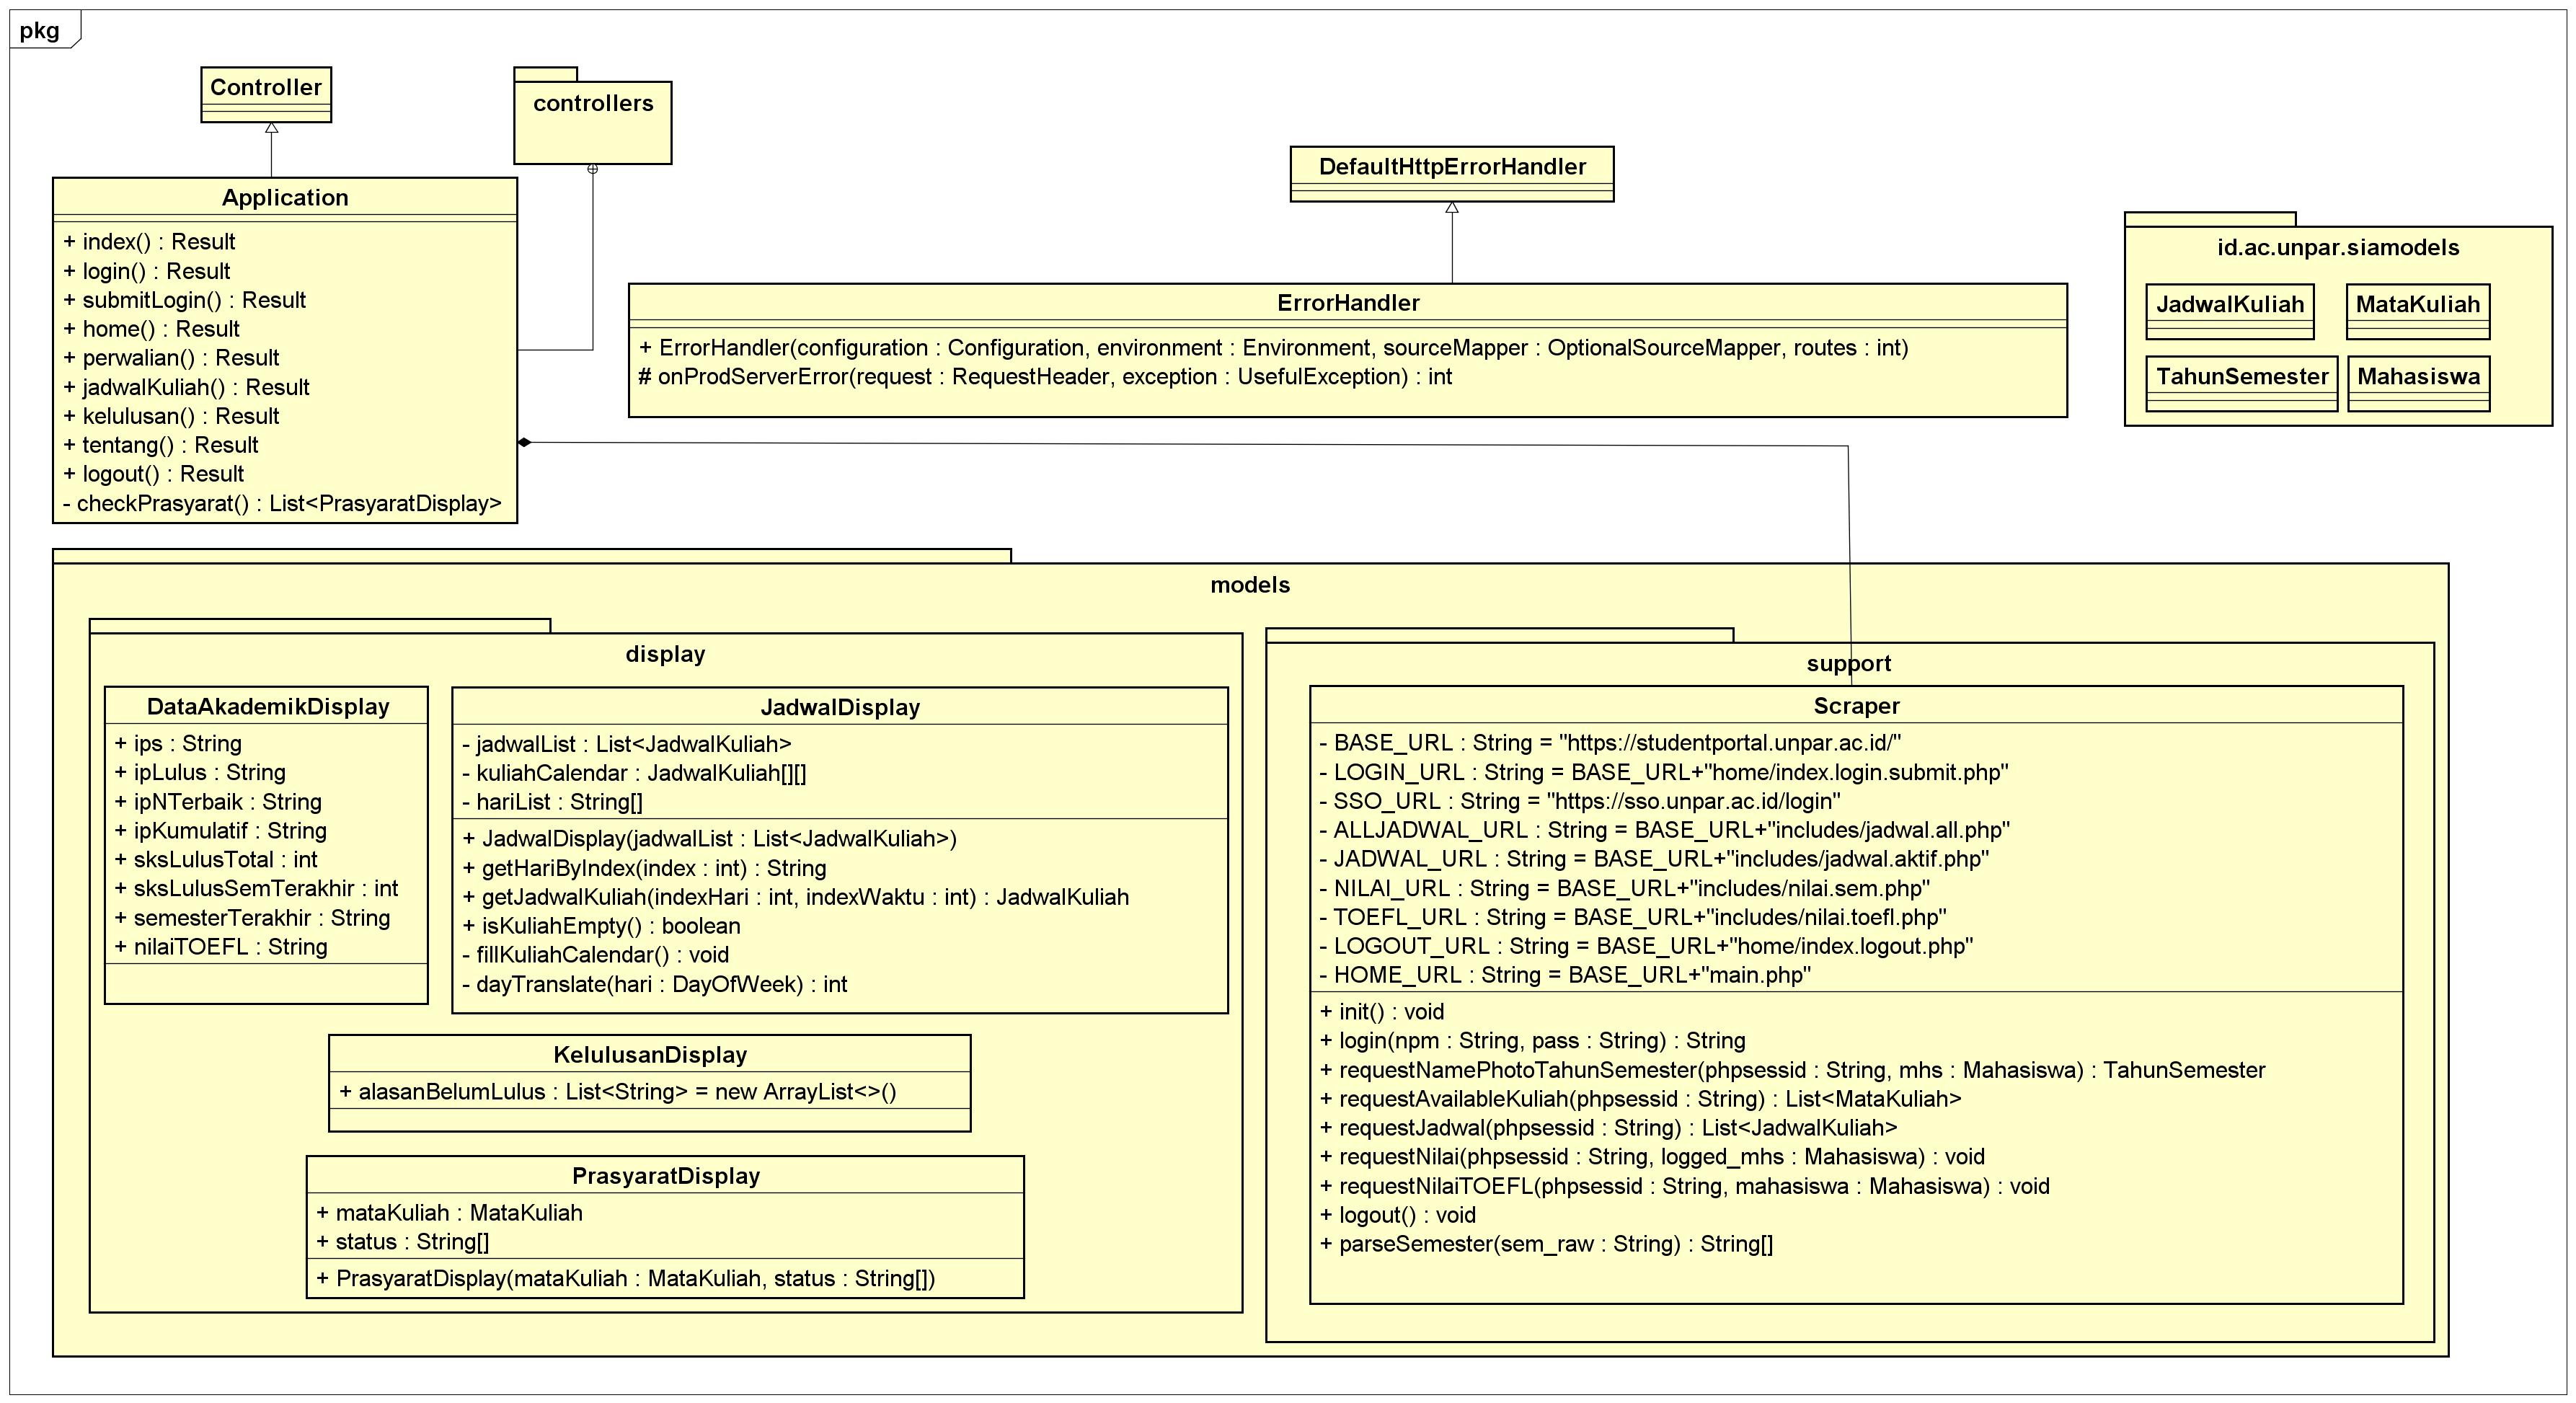
\includegraphics[scale=0.135]{Gambar/class-diagram-ifstudentportal}
			\caption{Diagram Kelas IFStudentPortal}
			\label{fig:2_ifstudentportal_class}
			\end{figure}

			\item \textbf{SIAModels} \\
			SIAModels merupakan kelas-kelas dalam bahasa Java yang merepresentasikan Sistem Informasi Akademik Teknik Informatika UNPAR. Saat ini SIAModels mendukung kurikulum 2013. Diagram kelas SIAModels dapat dilihat pada gambar \ref{fig:2_siamodels_class}.
			
			\begin{figure}[H]
			\centering
			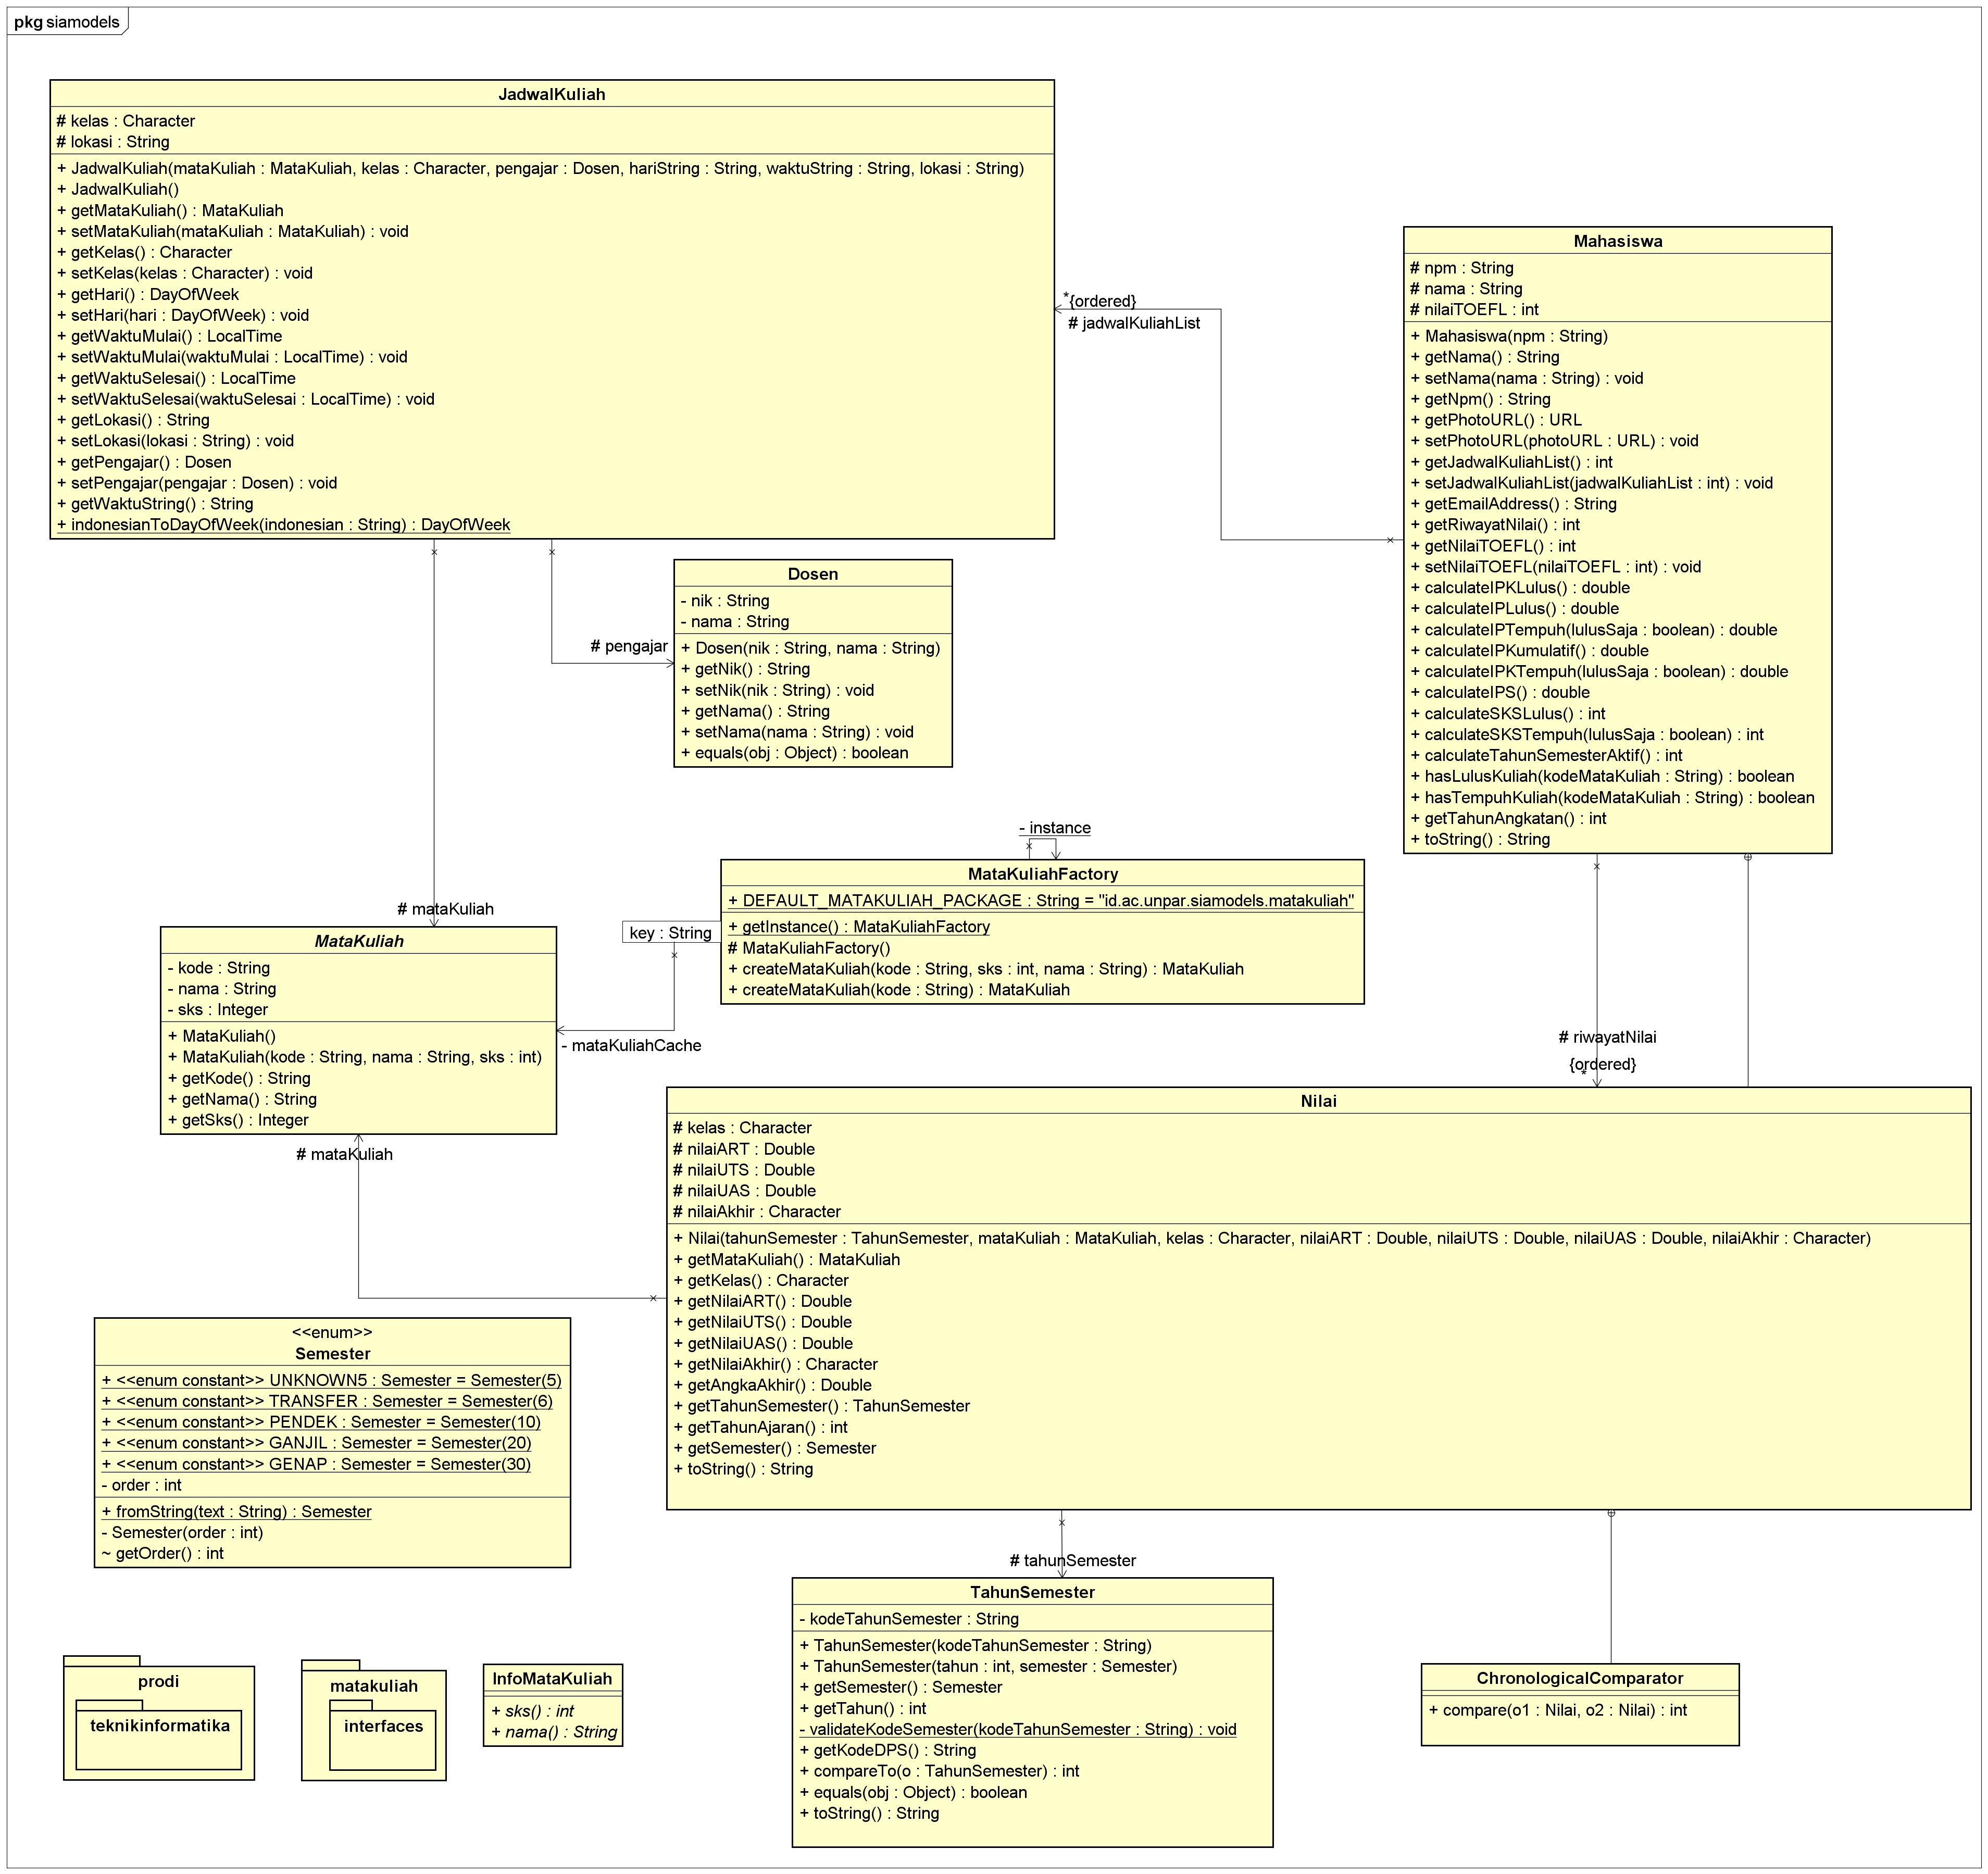
\includegraphics[scale=0.125]{Gambar/class-diagram-siamodels}
			\caption{Diagram Kelas SIAModels}
			\label{fig:2_siamodels_class}
			\end{figure}
		\end{enumerate}
		\item \textbf{Melakukan Studi Literatur mengenai Kurikulum 2018 dan Skripsi Herfan Heryandi}\\
		{\bf Status :} Ada sejak rencana kerja skripsi.\\
		{\bf Hasil :} Untuk studi literatur mengenai skripsi Herfan Heryandi dilakukan dengan membaca-baca hasil dokumen skripsinya dan studi literatur mengenai kurikulum 2018 dilakukan dengan membaca dokumen kurikulum 2018 versi 0.8 dan mencatatnya di dokumen skripsi pada bab 2. Beberapa hal dari dokumen kurikulum 2018 yang mempengaruhi perubahan pada SIAModels dan IFStudentPortal, yaitu :
		\begin{enumerate}
			\item \textbf{Struktur Kurikulum} \\
			Struktur Kurikulum 2018 dapat dilihat di Tabel \ref{tab:strukturkurikulum2018} \& \ref{tab:2_strukturkurikulum2018}.
			\begin{table}[H]
			\centering
				\caption{Struktur Kurikulum 2018 Program Studi Teknik Informatika(Semester 1-4)}
				\begin{tabular}{|p{0.5cm}|p{2.85cm}|p{4.95cm}|p{2.7cm}|p{2.7cm}|}
					\hline
					\multicolumn{1}{|c|}{\textbf{No}} & \multicolumn{1}{c|}{\textbf{Kode}} & \multicolumn{1}{c|}{\textbf{Mata Kuliah}} & \multicolumn{1}{c|}{\textbf{Bobot Koding}} & \multicolumn{1}{c|}{\textbf{SKS}} \\ \hline
					\multicolumn{5}{|l|}{\textbf{Semester 1}} \\ \hline
					1 &	AIF181101-03 &	Computational Thinking &	0.25 &	3   \\ \hline
					2 &	AIF181103-04 &	Matematika Dasar &	&	4  \\ \hline
					3 &	AIF181105-02 &	Pengantar Informatika &  & 2  \\ \hline
					4	& AIF181107-03 &	Matematika Diskret &	&	3  \\ \hline
					5	& MKU170130-02 &	Bahasa Indonesia &	&	2  \\ \hline
					6	& MKU170110-02 &	Pendidikan Kewarganegaraan &	&	2  \\ \hline
					7	& MKU170120-02 &	Logika &	&	2  \\ \hline
					\multicolumn{5}{|c|}{Wajib: 18 sks, Pilihan: -} \\ \hline
					\multicolumn{5}{|l|}{\textbf{Semester 2}} \\ \hline
					1 &	AIF181100-04 &	Dasar Pemrograman &	1 &	4 \\ \hline
					2 &	AIF181202-04 &	Arsitektur dan Organisasi Komputer & &	4  \\ \hline
					3 &	AIF181104-03 &	Logika Informatika &	0.25 &	3  \\ \hline
					4 &	AIF181106-03 &	Matriks dan Ruang Vektor &	0.25 &	3  \\ \hline
					5 &	MKU170240-02 &	Etika	& &	2  \\ \hline
					6 &	MKU170250-02 &	Pancasila & &	2  \\ \hline
					\multicolumn{5}{|c|}{Wajib: 18 sks, Pilihan: - }\\ \hline
					\multicolumn{5}{|l|}{\textbf{Semester 3}} \\ \hline
					1 &	AIF182101-03 &	Algoritma dan Struktur Data &	0.75 &	3  \\ \hline
					2 &	AIF182103-04 &	Struktur Diskret &	0.25 &	4  \\ \hline
					3 &	AIF182105-02 &	Pemrograman Berorientasi Objek &	1 &	2   \\ \hline
					4 &	AIF182007-02 &	Teknik Presentasi &  &	2  \\ \hline
					5 &	AIF182109-03 &	Statistika untuk Komputasi &	0.25 &	3  \\ \hline
					6 &	MKU170370-02 / MKU170380-02 &	Agama Katolik/Fenomenologi Agama & &	2  \\ \hline
					7 &	MKU170360-02 &	Estetika & &	2  \\ \hline
					\multicolumn{5}{|c|}{Wajib: 18 sks, Pilihan: -} \\ \hline
					\multicolumn{5}{|l|}{\textbf{Semester 4}} \\ \hline
					1	& AIF182100-04 &	Analisis Desain Berorientasi Objek &	0.75 &	4  \\ \hline
					2	& AIF182302-04 &	Majemen Informasi dan Basis Data &	0.75 &	4  \\ \hline
					3	& AIF182204-03 &	Pemrograman Berbasis Web &	1 &	3  \\ \hline
					4	& AIF182206-03 &	Sistem Operasi &	0.25 &	3  \\ \hline
					5 &	AIF182308-03 &	Pengantar Sistem Informasi &	0.25 &	3  \\ \hline
					6 &	- &	Pilihan &	&	2  \\ \hline
					\multicolumn{5}{|c|}{Wajib: 17 sks, Pilihan: 2 sks} \\ \hline
				\end{tabular}
			\label{tab:strukturkurikulum2018}
		\end{table}

		\begin{table}[H]
			\caption{Struktur Kurikulum 2018 Program Studi Teknik Informatika(Semester 5-8)}
			\centering
				\begin{tabular}{|p{0.5cm}|p{2.85cm}|p{4.95cm}|p{2.7cm}|p{2.7cm}|}
					\hline
					\multicolumn{1}{|c|}{\textbf{No}} & \multicolumn{1}{c|}{\textbf{Kode}} & \multicolumn{1}{c|}{\textbf{Mata Kuliah}} & \multicolumn{1}{c|}{\textbf{Bobot Koding}} & \multicolumn{1}{c|}{\textbf{SKS}} \\ \hline
					
					\multicolumn{5}{|l|}{\textbf{Semester 5}} \\ \hline
					1 &	AIF183101-03 &	Desain dan Analisis Algoritma &	0.75 &	3  \\ \hline
					2	& AIF183303-03 &	Rekayasa Perangkat Lunak &  &	3  \\ \hline
					3	& AIF183305-02 &	Manajemen Proyek &  &	2  \\ \hline
					4 &	AIF183307-02 &	Teknologi Basis Data &	0.75 &	2  \\ \hline
					5 &	AIF183209-03 &	Pemrograman Aplikasi Bergerak &	1 &	3 \\ \hline
					6 &	AIF183211-04 &	Jaringan Komputer &	0.25 &	4  \\ \hline
					7 &	- &	Pilihan &	&	2  \\ \hline
					\multicolumn{5}{|c|}{Wajib: 17 sks, Pilihan: 2 sks} \\ \hline
					\multicolumn{5}{|l|}{\textbf{Semester 6}} \\ \hline
					1	& AIF183100-03 &	Pengantar Sistem Cerdas &	0.25 &	3  \\ \hline
					2	& AIF183002-02 &	Penulisan Ilmiah &  &	2  \\ \hline
					3	& AIF183104-03 &	Interaksi Manusia Komputer &	0.5 &	3  \\ \hline
					4	& AIF183106-06 &	Proyek Informatika &	1 &	6 \\ \hline
						& AIF183308-03 &	Proyek Sistem Informasi 1	& 1 &	3  \\ \hline
					5	& - &	Pilihan &	&	4  \\ \hline
						& - &	Pilihan	& &	7  \\ \hline
					\multicolumn{5}{|c|}{Wajib: 14/11 sks, Pilihan: 4/7 sks} \\ \hline
					\multicolumn{5}{|l|}{\textbf{Semester 7}} \\ \hline
					1	& AIF184001-03	& Skripsi 1	& &	3  \\ \hline
					2	& AIF184303-03	& Proyek Sistem Informasi 2 &	1 &	3  \\ \hline
					3	& AIF184005-02	& Komputer dan Masyarakat &	&	2  \\ \hline
					4	& - &	Pilihan	& &	12  \\ \hline
						& - &	Pilihan	& &	9  \\ \hline
					\multicolumn{5}{|c|}{Wajib: 5/8 sks, Pilihan: 12/9 sks} \\ \hline
					\multicolumn{5}{|l|}{\textbf{Semester 8}} \\ \hline
					1 &	AIF184000-02 &	Etika Profesi &	&	2  \\ \hline
					2 &	AIF184002-05 &	Skripsi 2 &	0.75 &	5  \\ \hline
					 & AIF184004-08 &	Tugas Akhir &	0.75 &	8  \\ \hline
					3 &	- &	Pilihan	&  &	10/7  \\ \hline
					\multicolumn{5}{|c|}{Wajib: 7/10 sks, Pilihan: 10/7 sks} \\ \hline
				\end{tabular}
			\label{tab:2_strukturkurikulum2018}
		\end{table}
		
		\item \textbf{Kuliah Pilihan} \\
		Pada bagian ini, diberikan daftar mata kuliah pilihan pada Kurikulum 2018 ini. Daftar ini diberikan secara rinci pada Tabel \ref{tab:kuliahpilihan}.

\begin{table}[H]
	\centering
		\caption{Mata kuliah pilihan Program studi Teknik Informatika}
		\begin{tabular}{|p{0.5cm}|p{2.85cm}|p{4.95cm}|p{2.7cm}|}
			\hline
			\multicolumn{1}{|c|}{\textbf{No}} & \multicolumn{1}{c|}{\textbf{Kode}} & \multicolumn{1}{c|}{\textbf{Mata Kuliah}} & \multicolumn{1}{c|}{\textbf{SKS}} \\ \hline
\multicolumn{4}{|l|}{\textbf{Semester 4}}                                \\ \hline
1   & AIF182110-02    & Pemrograman Fungsional                     & 2   \\ \hline
2   & AIF182112-03    & Pemodelan Formal                           & 3   \\ \hline
3   & AIF182114-03    & Pemrograman Kompetitif 1                   & 3   \\ \hline
4   & AIF182116-02    & Dasar-dasar Java                           & 2   \\ \hline
5   & AIF182118-03    & Teori Bilangan                             & 3   \\ \hline
6   & AIF182120-02    & Teori Bahasa dan Kompilasi                 & 2   \\ \hline
7   & AIF182122-03    & Matematika Kombinatorial                   & 3   \\ \hline
8   & AIF182124-03    & Metode Numerik                             & 3   \\ \hline
9   & AIF182126-02    & Pemrograman Lojik                          & 2   \\ \hline

		\end{tabular}
	\label{tab:kuliahpilihan}
\end{table}

\begin{table}[H]
	\centering
		\begin{tabular}{|p{0.5cm}|p{2.85cm}|p{4.95cm}|p{2.7cm}|}
			\hline
			\multicolumn{1}{|c|}{\textbf{No}} & \multicolumn{1}{c|}{\textbf{Kode}} & \multicolumn{1}{c|}{\textbf{Mata Kuliah}} & \multicolumn{1}{c|}{\textbf{SKS}} \\ \hline
			\multicolumn{4}{|l|}{\textbf{Semester 5}}                                \\ \hline
1   & AIF183013-02    & Kerja Praktek 1                            & 2   \\ \hline
2   & AIF183015-03    & Pendidikan Pengabdian kepada Masyarakat    & 3   \\ \hline
3   & AIF183117-02    & Grafika Komputer                           & 2   \\ \hline
4   & AIF183119-02    & Keamanan Informasi                         & 2   \\ \hline
5   & AIF183121-03    & Pemrograman Kompetitif 2                   & 3   \\ \hline
6   & AIF183123-02    & Topik Khusus Informatika 1                 & 2   \\ \hline
7   & AIF183225-03    & Administrasi Jaringan Komputer 1           & 3   \\ \hline
8   & AIF183227-03    & Pengantar Telekomunikasi                   & 3   \\ \hline
9   & AIF183229-02    & Topik Khusus Sistem Terdistribusi 1        & 2   \\ \hline
			10  & AIF183331-03    & Sistem e-Commerce                          & 3   \\ \hline
11  & AIF183333-02    & Metodologi Pengembangan Sistem Informasi 1 & 2   \\ \hline
12  & AIF183337-02    & Topik Khusus Sistem Informasi 1            & 2   \\ \hline
\multicolumn{4}{|l|}{\textbf{Semester 6}}                                \\ \hline
1   & AIF183010-03    & Kerja Praktek 2                            & 3   \\ \hline
2   & AIF183112-02    & Pengujian Perangkat Lunak                  & 2   \\ \hline
3   & AIF183114-03    & Algoritma Kriptografi                      & 3   \\ \hline
4   & AIF183116-02    & Komputasi Paralel                          & 2   \\ \hline
5   & AIF183118-03    & Komputasi Geometri                         & 3   \\ \hline
6   & AIF183120-03    & Perancangan Permainan Komputer             & 3   \\ \hline
7   & AIF183122-03    & Pemodelan Simulasi                         & 3   \\ \hline
8   & AIF183124-03    & Grafika Komputer Lanjut                    & 3   \\ \hline
9   & AIF183126-03    & Pemrograman Kompetitif 3                   & 3   \\ \hline
10  & AIF183128-03    & Topik Khusus Informatika 2                 & 3   \\ \hline
11  & AIF183230-03    & Jaringan Komputer Lanjut                   & 3   \\ \hline
12  & AIF183232-03    & Pemrograman Berbasis Web Lanjut            & 3   \\ \hline
13  & AIF183234-03    & Sistem Aplikasi Telematika                 & 3   \\ \hline
14  & AIF183236-03    & Administrasi Jaringan Komputer 2           & 3   \\ \hline
15  & AIF183238-03    & Topik Khusus Sistem Terdistribusi 2        & 3   \\ \hline
16  & AIF183340-02    & Metodologi Pengembangan Sistem Informasi 1 & 2   \\ \hline
17  & AIF183342-03    & Kewirausahaan Berbasis Teknologi           & 3   \\ \hline
18 & AIF183346-03    & Topik Khusus Sistem Informasi 2            & 3   \\ \hline
19  & AIF183348-03    & Sistem Kecerdasan Bisnis                   & 3   \\ \hline
		\end{tabular}
	\label{tab:kuliahpilihan_2}
\end{table}

\begin{table}[H]
	\centering
		\begin{tabular}{|p{0.5cm}|p{2.85cm}|p{4.95cm}|p{2.7cm}|}
			\hline
			\multicolumn{1}{|c|}{\textbf{No}} & \multicolumn{1}{c|}{\textbf{Kode}} & \multicolumn{1}{c|}{\textbf{Mata Kuliah}} & \multicolumn{1}{c|}{\textbf{SKS}} \\ \hline
			\multicolumn{4}{|l|}{\textbf{Semester 7}}                                \\ \hline
1   & AIF184007-04    & Kerja Praktek 3                            & 4   \\ \hline
2   & AIF184109-03    & Pembelajaran Mesin                         & 3   \\ \hline
3   & AIF184115-02    & Pencarian dan Temu Kembali Informasi       & 2   \\ \hline
4   & AIF184119-03    & Kecerdasan Buatan untuk Permainan Komputer & 3   \\ \hline
5   & AIF184121-03    & Metode Optimisasi                          & 3   \\ \hline
6   & AIF184123-03    & Teknologi Mesin Pencari                    & 3   \\ \hline
7   & AIF184125-03    & Pengolahan Bahasa Alami                    & 3   \\ \hline
8   & AIF184127-03    & Topik Khusus Informatika 3                 & 3   \\ \hline
9   & AIF184129-03    & Administrasi Jaringan Komputer 3           & 3   \\ \hline
			10  & AIF184231-03    & Jaringan Nirkabel                          & 3   \\ \hline
			11  & AIF184233-03    & Teknologi Middleware                       & 3   \\ \hline
			12  & AIF184235-03    & Layanan Berbasis Web                       & 3   \\ \hline
13  & AIF184237-03    & Topik Khusus Sistem Terdistribusi 3        & 3   \\ \hline
14  & AIF184339-03    & Pengendalian dan Audit Teknologi Informasi & 3   \\ \hline
15  & AIF184341-03    & Penambangan Data                           & 3   \\ \hline
16  & AIF184343-03    & Topik Khusus Sistem Informasi 3            & 3   \\ \hline
17  & AIF184345-03  & Teknologi Big Data dan Cloud Computing     & 3   \\ \hline
\multicolumn{4}{|l|}{\textbf{Semester 8}}                                \\ \hline
1   & AIF184104-03    & Bio-Inspired Computing                     & 3   \\ \hline
2   & AIF184106-03    & Pemrograman Permainan Komputer             & 3   \\ \hline
3   & AIF184108-03    & Kompresi Data                              & 3   \\ \hline
4   & AIF184110-03    & Pengolahan Citra                           & 3   \\ \hline
5   & AIF184112-03    & Pemrosesan Data Geografis                  & 3   \\ \hline
6   & AIF184114-03    & Verifikasi Formal                          & 3   \\ \hline
7   & AIF184116-02    & Sistem Multi Agen                          & 2   \\ \hline
8   & AIF184118-02    & Pemrograman Sistem                         & 2   \\ \hline
9   & AIF184120-02    & Topik Khusus Informatika 4                 & 2   \\ \hline
10  & AIF184222-03    & Administrasi Jaringan Komputer 4           & 3   \\ \hline
11  & AIF184224-03    & Sistem Terdistribusi                       & 3   \\ \hline
12  & AIF184226-03    & Teknologi Multimedia                       & 3   \\ \hline
13  & AIF184228-02    & Pemrograman Jaringan                       & 2   \\ \hline
14  & AIF184230-03    & Keamanan Jaringan                          & 3   \\ \hline
15  & AIF184232-02    & Topik Khusus Sistem Terdistribusi 4        & 2   \\ \hline
16  & AIF184334-03    & Sistem Informasi Skala Besar               & 3   \\ \hline
17  & AIF184336-02    & Sistem e-Government                        & 2   \\ \hline
18  & AIF184338-03    & Manajemen Proses Bisnis                    & 3   \\ \hline
19  & AIF184340-03    & Sistem Informasi Geografis                 & 3   \\ \hline
20  & AIF184342-02    & Topik Khusus Sistem Informasi 4            & 2   \\ \hline
21  & AIF184344-03 & Analisis Big Data                          & 3   \\ \hline
		\end{tabular}
	\label{tab:kuliahpilihan_3}
\end{table}

			\item \textbf{Prasyarat Mata Kuliah} \\
				\begin{table}[H]
				\centering
		\caption{Daftar mata kuliah wajib dan prasyaratnya}
		\begin{tabular}{|p{0.5cm}|p{2.85cm}|p{4.95cm}|p{2.7cm}|p{2.7cm}|}
			\hline
			\multicolumn{1}{|c|}{\multirow{2}{*}{\textbf{No}}} & \multicolumn{1}{c|}{\multirow{2}{*}{\textbf{Kode}}} & \multicolumn{1}{c|}{\multirow{2}{*}{\textbf{Mata Kuliah}}} & \multicolumn{2}{c|}{\textbf{Mata Kuliah Prasyarat}} \\ \cline{4-5}
			 &  &  & \multicolumn{1}{c|}{\textbf{Tempuh}} & \multicolumn{1}{c|}{\textbf{Lulus}} \\ \hline
			\multicolumn{5}{|l|}{\textbf{Semester 1}} \\ \hline
1 & AIF181101-03 & Computational Thinking &  &  \\ \hline
2 & AIF181103-04 & Matematika Dasar &  &  \\ \hline
3 & AIF181105-02 & Pengantar Informatika &  &  \\ \hline
4 & AIF181107-03 & Matematika Diskret &  &  \\ \hline
5 & MKU170130-02 & Bahasa Indonesia &  &  \\ \hline
6 & MKU170110-02 & Pendidikan Kewarganegaraan &  &  \\ \hline
7 & MKU170120-02 & Logika &  &  \\ \hline
\multicolumn{5}{|l|}{\textbf{Semester 2}} \\ \hline
1 & AIF181100-04 & Dasar Pemrograman &  & AIF181101-03 \\ \hline
2 & AIF181202-04 & Arsitektur dan Organisasi Komputer &  &  \\ \hline
3 & AIF181104-03 & Logika Informatika &  &  \\ \hline
4 & AIF181106-03 & Matriks dan Ruang Vektor &  &  \\ \hline
5 & MKU170240-02 & Etika &  &  \\ \hline
6 & MKU170250-02 & Pancasila &  &  \\ \hline
\multicolumn{5}{|l|}{\textbf{Semester 3}} \\ \hline
1 & AIF182101-03 & Algoritma dan Struktur Data &  & AIF181100-04 \\ \hline
2 & AIF182103-04 & Struktur Diskret & AIF181107-03 &  \\ \hline
3 & AIF182105-02 & Pemrograman Berorientasi Objek &  & AIF181100-04 \\ \hline
4 & AIF182007-02 & Teknik Presentasi &  &  \\ \hline
5 & AIF182109-03 & Statistika untuk Komputasi &  &  \\ \hline
6 & MKU170370-02 / MKU170380-02 & Agama Katolik/Fenomenologi Agama &  &  \\ \hline
7 & MKU170360-02 & Estetika &  &  \\ \hline
\multicolumn{5}{|l|}{\textbf{Semester 4}} \\ \hline
1 & AIF182100-04 & Analisis Desain Berorientasi Objek &  & AIF182105-02 \\ \hline
2 & AIF182302-04 & Majemen Informasi dan Basis Data & AIF182101-03 &  \\ \hline
3 & AIF182204-03 & Pemrograman Berbasis Web & AIF182302-04 (bersamaan atau sudah tempuh) &  \\ \hline
4 & AIF182206-03 & Sistem Operasi & AIF182101-03 &  \\ \hline
5 & AIF182308-03 & Pengantar Sistem Informasi & AIF182302-04 (bersamaan atau sudah tempuh) & AIF181105-02 \\ \hline
		\end{tabular}
	\label{tab:DaftarMataKuliahWajibDanPrasyaratnya}
\end{table}

\begin{table}[H]
	\centering
		\begin{tabular}{|p{0.5cm}|p{2.85cm}|p{4.95cm}|p{2.7cm}|p{2.7cm}|}
			\hline
			\multicolumn{1}{|c|}{\multirow{2}{*}{\textbf{No}}} & \multicolumn{1}{c|}{\multirow{2}{*}{\textbf{Kode}}} & \multicolumn{1}{c|}{\multirow{2}{*}{\textbf{Mata Kuliah}}} & \multicolumn{2}{c|}{\textbf{Mata Kuliah Prasyarat}} \\ \cline{4-5}
			 &  &  & \multicolumn{1}{c|}{\textbf{Tempuh}} & \multicolumn{1}{c|}{\textbf{Lulus}} \\ \hline
			\multicolumn{5}{|l|}{\textbf{Semester 5}} \\ \hline
1 & AIF183101-03 & Desain dan Analisis Algoritma & AIF182103-04 & AIF182101-03 \\ \hline
2 & AIF183303-03 & Rekayasa Perangkat Lunak & AIF182100-04 &  \\ \hline
3 & AIF183305-02 & Manajemen Proyek & AIF183303-03 (bersamaan atau sudah tempuh) &  \\ \hline
4 & AIF183307-02 & Teknologi Basis Data &  & AIF182302-04 \\ \hline
5 & AIF183209-03 & Pemrograman Aplikasi Bergerak & AIF182100-04 &  \\ \hline
6 & AIF183211-04 & Jaringan Komputer & AIF182206-03 &  \\ \hline
\multicolumn{5}{|l|}{\textbf{Semester 6}} \\ \hline
1 & AIF183100-03 & Pengantar Sistem Cerdas & AIF183101-03 &  \\ 
 &  &  & AIF181104-03 &  \\ \hline
2 & AIF183002-02 & Penulisan Ilmiah &  &  \\ \hline
3 & AIF183104-03 & Interaksi Manusia Komputer &  &  \\ \hline
4 & AIF183106-06 & Proyek Informatika & AIF183303-03 &  \\ \hline
 & AIF183308-03 & Proyek Sistem Informasi 1 & AIF183305-02 & AIF182308-03 \\ \hline
\multicolumn{5}{|l|}{\textbf{Semester 7}} \\ \hline
1 & AIF184001-03 & Skripsi 1 &  & AIF183002-02 \\ 
 &  &  &  & AIF182007-02 \\ 
 &  &  &  & Sudah lulus 108 sks \\ \hline
2 & AIF184303-03 & Proyek Sistem Informasi 2 &  & AIF183308-03 \\ \hline
3 & AIF184005-02 & Komputer dan Masyarakat &  &  \\ \hline
\multicolumn{5}{|l|}{\textbf{Semester 8}} \\ \hline
1 & AIF184000-02 & Etika Profesi &  &  \\ \hline
2 & AIF184002-05 & Skripsi 2 &  & AIF184001-03 \\ 
 &  &  &  & Jika diambil bersamaan dengan AIF184001-03 \\ 
 &  &  &  & Prasyarat: lulus AIF183002-02 \\ 
 &  &  &  & AIF182007-02 \\
 &  &  &  & dan lulus 124 sks \\ \hline
3 & AIF184004-08 & Tugas Akhir &  & AIF183002-02 \\ 
 &  &  &  & AIF182007-02 \\
 &  &  &  & Sudah lulus 124 sks \\ \hline
		\end{tabular}
	\label{tab:DaftarMataKuliahWajibDanPrasyaratnya2}
\end{table}

\begin{table}[H]
	\centering
		\caption{Daftar mata kuliah pilihan dan prasyaratnya}
		\begin{tabular}{|p{0.5cm}|p{2.85cm}|p{4.95cm}|p{2.7cm}|p{2.7cm}|}
			\hline
			\multicolumn{1}{|c|}{\multirow{2}{*}{\textbf{No}}} & \multicolumn{1}{c|}{\multirow{2}{*}{\textbf{Kode}}} & \multicolumn{1}{c|}{\multirow{2}{*}{\textbf{Mata Kuliah}}} & \multicolumn{2}{c|}{\textbf{Mata Kuliah Prasyarat}} \\ \cline{4-5}
			 &  &  & \multicolumn{1}{c|}{\textbf{Tempuh}} & \multicolumn{1}{c|}{\textbf{Lulus}} \\ \hline
			\multicolumn{5}{|l|}{\textbf{Semester 4}} \\ \hline
1 & AIF182110-02 & Pemrograman Fungsional & AIF181107-03 &  \\ \hline
2 & AIF182112-03 & Pemodelan Formal &  & AIF181104-03 \\ \hline
3 & AIF182114-03 & Pemrograman Kompetitif 1 &  & AIF182101-03 (minimum C) \\ \hline
4 & AIF182116-02 & Dasar-dasar Java & AIF182105-02 &  \\ \hline
5 & AIF182118-03 & Teori Bilangan & AIF181107-03 &  \\ \hline
6 & AIF182120-02 & Teori Bahasa dan Kompilasi &  & AIF181104-03 \\
 &  &  &  & AIF182103-04 \\ \hline
7 & AIF182122-03 & Matematika Kombinatorial &  & AIF181107-03 \\ \hline
8 & AIF182124-03 & Metode Numerik &  & AIF181103-04 \\
 &  &  &  & AIF181100-04 \\ \hline
9 & AIF182126-02 & Pemrograman Lojik &  & AIF181104-03 \\ \hline
\multicolumn{5}{|l|}{\textbf{Semester 5}} \\ \hline
1 & AIF183013-02 & Kerja Praktek 1 &  &  \\ \hline
2 & AIF183015-03 & Pendidikan Pengabdian kepada Masyarakat &  &  \\ \hline
3 & AIF183117-02 & Grafika Komputer & AIF181103-04 & AIF182105-02 \\ \hline
4 & AIF183119-02 & Keamanan Informasi &  & AIF181107-03 \\ \hline
5 & AIF183121-03 & Pemrograman Kompetitif 2 &  & AIF182114-03 (minimum B) \\ \hline
6 & AIF183123-02 & Topik Khusus Informatika 1 &  &  \\ \hline
7 & AIF183225-03 & Administrasi Jaringan Komputer 1 &  &  \\ \hline
8 & AIF183227-03 & Pengantar Telekomunikasi & AIF183211-04 &  \\ \hline
9 & AIF183229-02 & Topik Khusus Sistem Terdistribusi 1 &  &  \\ \hline
10 & AIF183331-03 & Sistem e-Commerce &  & AIF182308-03 \\ \hline
11 & AIF183333-02 & Metodologi Pengembangan Sistem Informasi 1 &  & AIF182308-03 \\ \hline
12 & AIF183335-02 & Perencanaan Sistem Informasi &  & AIF182308-03 \\ \hline
13 & AIF183337-02 & Topik Khusus Sistem Informasi 1 &  &  \\ \hline
\multicolumn{5}{|l|}{\textbf{Semester 6}} \\ \hline
1 & AIF183010-03 & Kerja Praktek 2 &  &  \\ \hline
2 & AIF183112-02 & Pengujian Perangkat Lunak &  & AIF183303-03 \\ \hline
3 & AIF183114-03 & Algoritma Kriptografi & AIF183119-02 &  \\ \hline
4 & AIF183116-02 & Komputasi Paralel &  & AIF182101-03 \\ \hline
5 & AIF183118-03 & Komputasi Geometri &  & AIF183101-03 \\ \hline
6 & AIF183120-03 & Perancangan Permainan Komputer & AIF183117-02 &  \\ \hline
7 & AIF183122-03 & Pemodelan Simulasi & AIF182101-03 &  \\ \hline
8 & AIF183124-03 & Grafika Komputer Lanjut &  & AIF183117-02 \\ \hline
					\end{tabular}
	\label{tab:DaftarMataKuliahPilihanDanPrasyaratnya}
\end{table}

\begin{table}[H]
	\centering
		\begin{tabular}{|p{0.5cm}|p{2.85cm}|p{4.95cm}|p{2.7cm}|p{2.7cm}|}
			\hline
			\multicolumn{1}{|c|}{\multirow{2}{*}{\textbf{No}}} & \multicolumn{1}{c|}{\multirow{2}{*}{\textbf{Kode}}} & \multicolumn{1}{c|}{\multirow{2}{*}{\textbf{Mata Kuliah}}} & \multicolumn{2}{c|}{\textbf{Mata Kuliah Prasyarat}} \\ \cline{4-5}
			 &  &  & \multicolumn{1}{c|}{\textbf{Tempuh}} & \multicolumn{1}{c|}{\textbf{Lulus}} \\ \hline
			9 & AIF183126-03 & Pemrograman Kompetitif 3 &  & AIF183121-03 (minimum B) \\ \hline
10 & AIF183128-03 & Topik Khusus Informatika 2 &  &  \\ \hline
11 & AIF183230-03 & Jaringan Komputer Lanjut &  & AIF183211-04 \\ \hline
12 & AIF183232-03 & Pemrograman Berbasis Web Lanjut &  & AIF182204-03 \\
 &  &  &  & AIF182302-04 \\ \hline
13 & AIF183234-03 & Sistem Aplikasi Telematika &  & AIF183211-04 \\ \hline
14 & AIF183236-03 & Administrasi Jaringan Komputer 2 &  & AIF183225-03 \\ \hline
15 & AIF183238-03 & Topik Khusus Sistem Terdistribusi 2 &  &  \\ \hline
16 & AIF183340-02 & Metodologi Pengembangan Sistem Informasi 2 &  & AIF183331-02 \\ \hline
17 & AIF183342-03 & Kewirausahaan Berbasis Teknologi &  & Sudah lulus 90 sks \\ \hline
18 & AIF183346-03 & Topik Khusus Sistem Informasi 2 &  &  \\ \hline
19 & AIF183348-03 & Sistem Kecerdasan Bisnis & AIF182302-04 &  \\ \hline
\multicolumn{5}{|l|}{\textbf{Semester 7}} \\ \hline
1 & AIF184007-04 & Kerja Praktek 3 &  &  \\ \hline
2 & AIF184109-03 & Pembelajaran Mesin &  & AIF183100-03 \\ \hline
3 & AIF184115-02 & Pencarian dan Temu Kembali Informasi &  & AIF181103-04 \\ \hline
4 & AIF184119-03 & Kecerdasan Buatan untuk Permainan Komputer &  & AIF183100-03 \\ \hline
5 & AIF184121-03 & Metode Optimisasi & AIF183100-03 & AIF183101-03 \\ \hline
6 & AIF184123-03 & Teknologi Mesin Pencari & AIF181106-03 &  \\ \hline
7 & AIF184125-03 & Pengolahan Bahasa Alami &  & AIF183100-03 \\ \hline
8 & AIF184127-03 & Topik Khusus Informatika 3 &  &  \\ \hline
9 & AIF184129-03 & Administrasi Jaringan Komputer 3 &  & AIF183234-03 \\ \hline
10 & AIF184231-03 & Jaringan Nirkabel &  & AIF183211-04 \\ \hline
11 & AIF184233-03 & Teknologi Middleware &  & AIF183211-04 \\ \hline
12 & AIF184235-03 & Layanan Berbasis Web &  & AIF182204-03 \\
 &  &  &  & AIF182302-04 \\
 &  &  &  & AIF183211-04 \\ \hline
13 & AIF184237-03 & Topik Khusus Sistem Terdistribusi 3 &  &  \\ \hline
14 & AIF184339-03 & Pengendalian dan Audit Teknologi Informasi & AIF182308-03 &  \\ \hline
15 & AIF184341-03 & Penambangan Data &  & AIF182101-03 \\ \hline
16 & AIF184343-03 & Topik Khusus Sistem Informasi 3 &  &  \\ \hline
17 & AIF184345-03 & Teknologi Big Data dan Cloud Computing &  & AIF183307-02 dan AIF183211-04 \\ \hline
		\end{tabular}
	\label{tab:DaftarMataKuliahPilihanDanPrasyaratnya2}
\end{table}

\begin{table}[H]
	\centering
		\begin{tabular}{|p{0.5cm}|p{2.85cm}|p{4.95cm}|p{2.7cm}|p{2.7cm}|}
			\hline
			\multicolumn{1}{|c|}{\multirow{2}{*}{\textbf{No}}} & \multicolumn{1}{c|}{\multirow{2}{*}{\textbf{Kode}}} & \multicolumn{1}{c|}{\multirow{2}{*}{\textbf{Mata Kuliah}}} & \multicolumn{2}{c|}{\textbf{Mata Kuliah Prasyarat}} \\ \cline{4-5}
			 &  &  & \multicolumn{1}{c|}{\textbf{Tempuh}} & \multicolumn{1}{c|}{\textbf{Lulus}} \\ \hline
\multicolumn{5}{|l|}{\textbf{Semester 8}} \\ \hline
1 & AIF184104-03 & Bio-Inspired Computing &  & AIF183101-03 \\ \hline
2 & AIF184106-03 & Pemrograman Permainan Komputer &  & AIF182100-04 \\ \hline
3 & AIF184108-03 & Kompresi Data &  & AIF183101-03 \\ \hline
4 & AIF184110-03 & Pengolahan Citra &  & AIF181106-03 \\ \hline
5 & AIF184112-03 & Pemrosesan Data Geografis &  & AIF182101-03 \\ \hline
6 & AIF184114-03 & Verifikasi Formal &  & AIF184117-02 \\ \hline
7 & AIF184116-02 & Sistem Multi Agen & AIF182206-03 &  \\
 &  &  & AIF183100-03 &  \\ \hline
8 & AIF184118-02 & Pemrograman Sistem & AIF182206-03 & AIF181100-04 \\ \hline
9 & AIF184120-02 & Topik Khusus Informatika 4 &  &  \\ \hline
10 & AIF184222-03 & Administrasi Jaringan Komputer 4 &  & AIF184129-03 \\ \hline
11 & AIF184224-03 & Sistem Terdistribusi &  & AIF183211-04 \\ \hline
12 & AIF184226-03 & Teknologi Multimedia &  & AIF183104-03 \\ \hline
13 & AIF184228-02 & Pemrograman Jaringan &  & AIF183211-04 \\ \hline
14 & AIF184230-03 & Keamanan Jaringan & AIF183119-02 &  \\ \hline
15 & AIF184232-02 & Topik Khusus Sistem Terdistribusi 4 &  &  \\ \hline
16 & AIF184334-03 & Sistem Informasi Skala Besar &  & AIF182308-03 \\ \hline
17 & AIF184336-02 & Sistem e-Government &  &  \\ \hline
18 & AIF184338-03 & Manajemen Proses Bisnis & AIF182105-02 &  \\
 &  &  & AIF182204-03 &  \\ \hline
19 & AIF184340-02 & Sistem Informasi Geografis &  & AIF182308-03 \\ \hline
20 & AIF184342-02 & Topik Khusus Sistem Informasi 4 &  &  \\ \hline
21 & AIF184344-03 & Analisis Big Data & AIF184341-03 & \\  \hline
		\end{tabular}
	\label{tab:DaftarMataKuliahPilihanDanPrasyaratnya3}
\end{table}

			\item \textbf{Angka Akhir dan Konversinya} \\
			
			\begin{table}[H]
				\centering
				\caption{Angka akhir dan konversinya}
					\begin{tabular}{|c|c|c|}
						\hline
						Angka Akhir (AA) & Nilai Akhir (NA) & Bobot Nilai Akhir \\ \hline
						80-100         & A                & 4                 \\ \hline
						77-79          & A-               & 3.67              \\ \hline
						73-76          & B+               & 3.33              \\ \hline
						70-72          & B                & 3                 \\ \hline
						67-69          & B-               & 2.67              \\ \hline
						63-66          & C+               & 2.33              \\ \hline
						60-62          & C                & 2                 \\ \hline
						57-59          & C-               & 1.67              \\ \hline
						50-56          & D                & 1                 \\ \hline
						0-49           & E                & 0                 \\ \hline
					\end{tabular}
				\label{tab:AngkaAkhirDanKonversinya}
			\end{table}
			
			\item \textbf{Syarat Kelulusan} \\ 
			Syarat kelulusan pada Kurikulum 2018 bagi mahasiswa Prodi Teknik Informatika UNPAR adalah:
			\begin{enumerate}
				\item Memenuhi syarat kelulusan sarjana yang diterapkan oleh universitas.
				\item Lulus minimal 144 SKS dengan IPK minimal 2.0, dengan ketentuan berikut:
				\begin{enumerate}
					\item Lulus (minimal dengan nilai D) di semua mata kuliah wajib.
					\item Lulus dengan nilai minimal C pada mata kuliah Skripsi 1 dan Skripsi 2.
					\item Lulus pada salah satu jalur kuliah proyek (Proyek Informatika atau Proyek Sistem Informasi 1 dan Sistem Informasi 2).
					\item Mengambil maksimum 10 sks mata kuliah pilihan dari luar Prodi Teknik Informatika.
				\end{enumerate}
				\item Aturan kelulusan lainnya mengikuti aturan konversi yang berlaku.
			\end{enumerate}
			
			\item \textbf{Transisi Kurikulum} \\
				\begin{itemize}
					\item \textbf{Daftar Mata Kuliah Yang Tidak Wajib lulus perangkatan} \\
					\begin{table}[H]
					\centering
					\caption{Daftar mata kuliah wajib yang tidak wajib lulus per angkatan}
					\label{tab:2_wajibtidaklulus}
					\begin{tabular}{|c|c|p{3.25cm}|c|c|c|c|c|c|c|}
					\hline
					\multicolumn{1}{|c|}{\multirow{2}{*}{\textbf{No}}} & \multicolumn{1}{c|}{\multirow{2}{*}{\textbf{Kode}}} & \multicolumn{1}{c|}{\multirow{2}{*}{\textbf{Mata Kuliah}}} & \multicolumn{7}{c|}{\textbf{Angkatan TIDAK wajib lulus}} \\ \cline{4-10} 
					\multicolumn{1}{|c|}{} & \multicolumn{1}{c|}{} & \multicolumn{1}{c|}{} & \textbf{2011} & \textbf{2012} & \textbf{2013} & \textbf{2014} & \textbf{2015} & \textbf{2016} & \textbf{2017} \\ \hline
					1 & AIF181101-03 & Computational Thinking & v & v & v & v & v & v & v \\ \hline
					2 & AIF181100-04 & Dasar Pemrograman & v & v &  &  &  &  &  \\ \hline
					3 & AIF181106-03 & Matriks dan Ruang Vektor & v & v & v & v & v & v & v \\ \hline
					4 & AIF182007-02 & Teknik Presentasi & v & v & v & v & v & v &  \\ \hline
					5 & AIF182204-03 & Pemrograman Berbasis Web & v & v & v & v & v & v &  \\ \hline
					6 & AIF183307-02 & Teknologi Basis Data & v & v & v & v & v &  &  \\ \hline
					7 & AIF183305-02 & Manajemen Proyek & v & v & v & v & v &  &  \\ \hline
					8 & AIF183209-03 & Pemrograman Aplikasi Bergerak & v & v & v & v & v &  &  \\ \hline
					\end{tabular}
					\end{table}
					
					\item \textbf{Aturan Kelulusan Perangkatan} \\
					\begin{table}[H]
					\centering
					\caption{Aturan kelulusan per angkatan}
					\label{tab:AturanKelulusan}
					\begin{tabular}{|p{2.5cm}|p{3.5cm}|p{3.5cm}|p{3.5cm}|}
					\hline
					\textbf{Angkatan} & \textbf{Jumlah sks lulus (min.) kuliah wajib prodi} & \textbf{Jumlah sks lulus MKU} & \textbf{Mata kuliah pilihan wajib Kurikulum 2013 (buah)} \\ \hline
					2011 & 78 & 14 & 3 \\ \hline
					2012 & 78 & 14 & 3 \\ \hline
					2013 & 82 & 14 & 3 \\ \hline
					2014 & 82 & 14 & 3 \\ \hline
					2015 & 82 & 14 & 0 \\ \hline
					2016 & 93 & 14 & 0 \\ \hline
					2017 & 98 & 14 & 0 \\ \hline
					\end{tabular}
					\end{table}
					
					\item \textbf{Daftar mata kuliah transisi}\\
					\begin{table}[H]
						\centering
							\caption{Daftar mata kuliah transisi}
							\begin{tabular}{|p{2.85cm}|p{7.95cm}|p{1.75cm}|}
								\hline
								\multicolumn{1}{|c|}{\textbf{Kode}} & \multicolumn{1}{c|}{\textbf{Mata Kuliah}} & \multicolumn{1}{c|}{\textbf{SKS}} \\ \hline
								\multicolumn{3}{|l|}{\textbf{Semester 1}}                    \\ \hline
					AIF181091-02 & Bahasa Inggris                          & 2   \\ \hline
					AIF182195-01 & Praktika Pemrograman Berorientasi Objek & 1   \\ \hline
					AIF181195-03 & Pengantar Informatika                   & 3   \\ \hline
					AIF181193-03 & Matematika Dasar                        & 3   \\ \hline
					\multicolumn{3}{|l|}{\textbf{Semester 2}}                    \\ \hline
					AIF182191-01 & Praktika Algoritma dan Struktur Data    & 1   \\ \hline
					AIF181298-03 & Sistem Dijital                          & 3   \\ \hline
					AIF181194-02 & Logika Informatika                      & 2   \\ \hline
					AIF182190-03 & Analisis Desain Berorientasi  Objek     & 3   \\ \hline
					\multicolumn{3}{|l|}{\textbf{Semester 4}}                    \\ \hline
					AIF183191-01 & Praktika Desain dan Analisis Algoritma  & 1   \\ \hline
					AIF182296-01 & Praktika Sistem Operasi                 & 1   \\ \hline
					AIF183393-04 & Rekayasa Perangkat Lunak                & 4   \\ \hline
					AIF182392-03 & Manajemen Informasi dan Basis Data      & 3   \\ \hline
					AIF183194-02 & Interaksi Manusia Komputer              & 2   \\ \hline
					\multicolumn{3}{|l|}{\textbf{Semester 5}}                    \\ \hline
					AIF183195-02 & Desain Antarmuka Grafis                 & 2   \\ \hline
					AIF183197-03 & Matematika Teknik                       & 3   \\ \hline
					AIF182294-02 & Pemrograman Berbasis Web                & 2   \\ \hline
					AIF183393-02 & Analisis Sistem Informasi               & 2   \\ \hline
					\multicolumn{3}{|l|}{\textbf{Semester 6}}                    \\ \hline
					AIF183290-02 & Analisis Proses Bisnis                  & 2   \\ \hline
					AIF183299-02

					 & Pemrograman Aplikasi Bergerak           & 2   \\ \hline
					AIF184191-02 & Algoritma Genetika                      & 2   \\ \hline
					AIF184193-02 & Jaringan Syaraf Tiruan                  & 2   \\ \hline
					\multicolumn{3}{|l|}{\textbf{Semester 7}}                    \\ \hline
					AIF184091-04 & Skripsi 1                               & 4   \\ \hline
					AIF184197-02 & Metode Formal                           & 2   \\ \hline
					AIF183390-03 & Sistem Pendukung Keputusan              & 3   \\ \hline
					AIF183395-02 & Perencanaan Sistem Informasi            & 2   \\ \hline
					\multicolumn{3}{|l|}{\textbf{Semester 8}}                    \\ \hline
					AIF184092-06 & Skripsi 2                               & 6   \\ \hline
					AIF184390-02 & Sistem Perusahaan Berskala Besar        & 2   \\ \hline
							\end{tabular}
						\label{tab:MataKuliahTransisi}
					\end{table}
					
					\item \textbf{Aturan konversi mata kuliah wajib dan pilihan wajib}\\
					\begin{table}[H]
						\centering
						\caption{Aturan konversi mata kuliah wajib dan pilihan wajib}
						\label{tab:aturankonversiwajib}
						\begin{tabular}{|p{0.35cm}|p{2cm}|p{0.55cm}|p{3.45cm}|p{2.65cm}|p{0.55cm}|p{3.45cm}|}
						\hline
						\multicolumn{1}{|c|}{} & \multicolumn{3}{c|}{\textbf{Kurikulum 2013/2008}} & \multicolumn{3}{c|}{\textbf{Kurikulum 2018}} \\ \cline{2-7} 
						\multicolumn{1}{|c|}{\multirow{-2}{*}{\textbf{No}}} & \multicolumn{1}{c|}{\textbf{Kode}} & \multicolumn{1}{c|}{\textbf{SKS}} & \multicolumn{1}{c|}{\textbf{Mata Kuliah}} & \multicolumn{1}{c|}{\textbf{Kode}} & \multicolumn{1}{c|}{\textbf{SKS}} & \multicolumn{1}{c|}{\textbf{Mata Kuliah}} \\ \hline
						\multicolumn{7}{|l|}{\textbf{Semester 1}} \\ \hline
						1 & MKU 010 & 2 & Bahasa Inggris & AIF181091-02 & 2 & Bahasa Inggris \\ \hline
						2 & MKU 008 & 2 & Etika & MKU170240-02 & 2 & Etika \\ \hline
						3 & MKU 001 & 2 & Pendidikan Pancasila & MKU170250-02 & 2 & Pendidikan Pancasila \\ \hline
						 & \multicolumn{1}{c|}{} &  &  & AIF181100-04 & 4 & Dasar Pemrograman \\ \cline{5-7} 
						 & \multicolumn{1}{c|}{\multirow{-2}{*}{AIF 101}} & \multirow{-2}{*}{6} &  & AIF182105-02 & 2 & Pemrograman Berorientasi Objek \\ \cline{2-3} \cline{5-7} 
						 & \multicolumn{1}{c|}{} &  &  & AIF182105-02 & 2 & Pemrograman Berorientasi Objek \\ \cline{5-7} 
						\multirow{-4}{*}{4} & \multicolumn{1}{c|}{\multirow{-2}{*}{AIF 191}} & \multirow{-2}{*}{3} & \multirow{-4}{*}{ \shortstack[l]{Pemrograman \\ Berorientasi Objek}} & AIF182195-01 & 1 & Praktika Pemrograman Berorientasi Objek \\ \hline
						
						
						\end{tabular}
						\end{table}

						\begin{table}[H]
						\centering
						\label{tab:aturankonversiwajib_2}
						\begin{tabular}{|p{0.35cm}|p{2cm}|p{0.55cm}|p{3.45cm}|p{2.65cm}|p{0.55cm}|p{3.45cm}|}
						\hline
						\multicolumn{1}{|c|}{} & \multicolumn{3}{c|}{\textbf{Kurikulum 2013/2008}} & \multicolumn{3}{c|}{\textbf{Kurikulum 2018}} \\ \cline{2-7} 
						\multicolumn{1}{|c|}{\multirow{-2}{*}{\textbf{No}}} & \multicolumn{1}{c|}{\textbf{Kode}} & \multicolumn{1}{c|}{\textbf{SKS}} & \multicolumn{1}{c|}{\textbf{Mata Kuliah}} & \multicolumn{1}{c|}{\textbf{Kode}} & \multicolumn{1}{c|}{\textbf{SKS}} & \multicolumn{1}{c|}{\textbf{Mata Kuliah}} \\ \hline
						 & AIF 105 & 3 &  & AIF181195-03 & 3 & Pengantar Informatika \\ \cline{2-3} \cline{5-7} 
						\multirow{-2}{*}{5} & AIF 195 & 2 & \multirow{-2}{*}{\shortstack[l]{Pengantar \\ Informatika}} & AIF181105-02 & 2 & Pengantar Informatika \\ \hline
						6 & AIF 103 & 3 & Matematika Diskret & AIF181107-03 & 3 & Matematika Diskret \\ \hline
						\multicolumn{7}{|l|}{\textbf{Semester 2}} \\ \hline
						1 & MKU 009 & 2 & Bahasa Indonesia & MKU170130-02 & 2 & Bahasa Indonesia \\ \hline
						2 & MKU 011 & 2 & Estetika & MKU170360-02 & 2 & Estetika \\ \hline
						 &  &  &  & AIF182101-03 & 3 & Algoritma dan Struktur Data \\ \cline{5-7} 
						 & \multirow{-2}{*}{AIF 102} & \multirow{-2}{*}{4} &  & AIF182191-01 & 1 & Praktika Algoritma dan Staruktur Data \\ \cline{2-3} \cline{5-7} 
						\multirow{-3}{*}{3} & AIF 192 & 3 & \multirow{-3}{*}{\shortstack[l]{Algoritma dan \\ Struktur Data}} & AIF182101-03 & 3 & Algoritma dan Struktur Data \\ \hline
						 & AMS100 & 4 &  & AIF181103-04 & 4 &  \\ \cline{2-3} \cline{5-6}
						\multirow{-2}{*}{4} & AMS190 & 3 & \multirow{-2}{*}{\shortstack[l]{Matematika \\ Informatika}} & AIF181193-03 & 3 & \multirow{-2}{*}{Matematika Dasar} \\ \hline
						5 & AIF 106 & 3 & Sistem Dijital & AIF181298-03 & 3 & Sistem Dijital \\ \hline
						 & AIF 104 & 3 &  & AIF181104-03 & 3 &  \\ \cline{2-3} \cline{5-6}
						\multirow{-2}{*}{6} & AIF 198 & 2 & \multirow{-2}{*}{Logika Informatika} & AIF181194-02 & 2 & \multirow{-2}{*}{Logika Informatika} \\ \hline
						\multicolumn{7}{|l|}{\textbf{Semester 3}} \\ \hline
						1 & MKU 012 & 2 & Logika & MKU170120-02 & 2 & Logika \\ \hline
						2 & MKU 003 & 2 & Agama Katolik & MKU170370-02 & 2 & Agama Katolik \\ \hline
						3 & MKU 004 & 2 & Fenomenologi Agama & MKU170380-02 & 2 & Fenomenologi Agama \\ \hline
						4 & AMS 200 & 3 & Probabilitas dan Statistika & AIF182109-03 & 3 & Statistika untuk Komputasi \\ \hline
						 & AIF 201 & 4 &  & AIF182100-04 & 4 &  \\ \cline{2-3} \cline{5-6}
						\multirow{-2}{*}{5} & AIF292 & 3 & \multirow{-2}{*}{\shortstack[l]{Analisis Desain \\ Berorientasi Objek}} & AIF182190-03 & 3 & \multirow{-2}{*}{\shortstack[l]{Analisis Desain \\ Berorientasi Objek}} \\ \hline
						6 & AIF 203 & 4 & Struktur Diskret & AIF182103-04 & 4 & Struktur Diskret \\ \hline
						7 & AIF 205 & 3 & Arsitektur dan Organisasi Komputer & AIF181202-04 & 4 & Arsitektur dan Organisasi Komputer \\ \hline
						\multicolumn{7}{|l|}{\textbf{Semester 4}} \\ \hline
						 &  &  &  & AIF183101-03 & 3 & Desain dan Analisis Algoritma \\ \cline{5-7} 
						 & \multirow{-2}{*}{AIF 202} & \multirow{-2}{*}{4} &  & AIF183191-01 & 1 & Praktika Desain dan Analisis Algoritma \\ \cline{2-3} \cline{5-7} 
						\multirow{-3}{*}{1} & AIF 292 & 3 & \multirow{-3}{*}{\shortstack[l]{Desain dan Analisis \\ Algoritma}} & AIF183101-03 & 3 & Desain dan Analisis Algoritma \\ \hline
						 & AIF 204 & 4 &  & AIF182302-04 & 4 &  \\ \cline{2-3} \cline{5-6}
						\multirow{-2}{*}{2} & AIF 294 & 3 & \multirow{-2}{*}{\shortstack[l]{Manajemen Info-\\rmasi dan Basisdata}} & AIF182392-03 & 3 & \multirow{-2}{*}{\shortstack[l]{Manajemen Info-\\rmasi dan Basisdata}} \\ \hline
						 &  &  &  & AIF182206-03 & 3 & Sistem Operasi \\ \cline{5-7} 
						 & \multirow{-2}{*}{AIF 206} & \multirow{-2}{*}{4} &  & AIF182296-01 & 1 & Praktika Sistem Operasi \\ \cline{2-3} \cline{5-7} 
						\multirow{-3}{*}{3} & AIF 296 & 3 & \multirow{-3}{*}{Sistem Operasi} & AIF182206-03 & 3 & Sistem Operasi \\ \hline
						 & AIF 208 & 4 &  & AIF183393-04 & 4 & Rekayasa Perangkat Lunak \\ \cline{2-3} \cline{5-7} 
						\multirow{-2}{*}{4} & AIF 298 & 3 & \multirow{-2}{*}{\shortstack[l]{Rekayasa Perangkat \\ Lunak}} & AIF183303-03 & 3 & Rekayasa Perangkat Lunak \\ \hline
						 & AIF 210 & 2 &  & AIF183194-02 & 2 &  \\ \cline{2-3} \cline{5-6}
						\multirow{-2}{*}{5} & AIF 290 & 3 & \multirow{-2}{*}{\shortstack[l]{Interaksi Manusia \\ Komputer}} & AIF183104-03 & 3 & \multirow{-2}{*}{\shortstack[l]{Interaksi Manusia \\ Komputer}} \\ \hline
						\end{tabular}
						\end{table}

						\begin{table}[H]
						\centering
						\label{tab:aturankonversiwajib_3}
						\begin{tabular}{|p{0.35cm}|p{2cm}|p{0.55cm}|p{3.45cm}|p{2.65cm}|p{0.55cm}|p{3.45cm}|}
						\hline
						\multicolumn{1}{|c|}{} & \multicolumn{3}{c|}{\textbf{Kurikulum 2013/2008}} & \multicolumn{3}{c|}{\textbf{Kurikulum 2018}} \\ \cline{2-7} 
						\multicolumn{1}{|c|}{\multirow{-2}{*}{\textbf{No}}} & \multicolumn{1}{c|}{\textbf{Kode}} & \multicolumn{1}{c|}{\textbf{SKS}} & \multicolumn{1}{c|}{\textbf{Mata Kuliah}} & \multicolumn{1}{c|}{\textbf{Kode}} & \multicolumn{1}{c|}{\textbf{SKS}} & \multicolumn{1}{c|}{\textbf{Mata Kuliah}} \\ \hline
						\multicolumn{7}{|l|}{\textbf{Semester 5}} \\ \hline
						1 & MKU 002 & 2 & Pendidikan Kewarganegaraan & MKU170110-02 & 2 & Pendidikan Kewarganegaraan \\ \hline
						2 & AIF 301 & 3 & Pengantar Sistem Cerdas & AIF183100-03 & 3 & Pengantar Sistem Cerdas \\ \hline
						3 & AIF 303 & 3 & Pengantar Sistem Informasi & AIF182308-03 & 3 & Pengantar Sistem Informasi \\ \hline
						4 & AIF 305 & 4 & Jaringan Komputer & AIF183211-04 & 4 & Jaringan Komputer \\ \hline
						5 & AIF 311 & 2 & Pemrograman Fungsional & AIF182110-02 & 2 & Pemrograman Fungsional \\ \hline
						6 & AIF 313 & 2 & Grafika Komputer & AIF183117-02 & 2 & Grafika Komputer \\ \hline
						7 & AIF 315 & 2 & Pemrograman Berbasis Web & AIF182294-02 & 2 & Pemrograman Berbasis Web \\ \hline
						8 & AIF 317 & 2 & Desain Antarmuka Grafis & AIF183191-02 & 2 & Desain Antarmuka Grafis \\ \hline
						\multicolumn{7}{|l|}{\textbf{Semester 6}} \\ \hline
						1 & AIF 302 & 2 & Penulisan Ilmiah & AIF183002-02 & 2 & Penulisan Ilmiah \\ \hline
						2 & AIF 304 & 3 & Proyek Sistem Informasi 1 & AIF183308-03 & 3 & Proyek Sistem Informasi 1 \\ \hline
						3 & AIF 306 & 6 & Proyek Informatika & AIF183106-06 & 6 & Proyek Informatika \\ \hline
						4 & AIF 312 & 2 & Keamanan Informasi & AIF183119-02 & 2 & Keamanan Informasi \\ \hline
						5 & AIF 314 & 2 & Pemrograman Basisdata & AIF183307-02 & 2 & Teknologi Basisdata \\ \hline
						6 & AIF 316 & 2 & Komputasi Paralel & AIF183116-02 & 2 & Komputasi Paralel \\ \hline
						7 & AIF 318 & 2 & Pemrograman Aplikasi Bergerak & AIF183299-02 & 2 & Pemrograman Aplikasi Bergerak \\ \hline
						\multicolumn{7}{|l|}{\textbf{Semester 7}} \\ \hline
						1 & AIF 401 & 4 & Skripsi 1 & AIF184091-04 & 4 & Skripsi 1 \\ \hline
						2 & AIF 403 & 3 & Proyek Sistem Informasi 2 & AIF184303-03 & 3 & Proyek Sistem Informasi 2 \\ \hline
						3 & AIF 405 & 2 & Komputer dan Masyarakat & AIF184005-02 & 2 & Komputer dan Masyarakat \\ \hline
						\multicolumn{7}{|l|}{\textbf{Semester 8}} \\ \hline
						1 & APS 402 & 2 & Etika Profesi & AIF184000-02 & 2 & Etika Profesi \\ \hline
						2 & AIF 402 & 6 & Skripsi 2 & AIF184092-06 & 6 & Skripsi 2 \\ \hline
						\end{tabular}
						\end{table}
				\end{itemize}
		\end{enumerate}

		\item \textbf{Melakukan konvesi nilai-nilai mata kuliah kurikulum 2013 ke kurikulum 2018}\\
		{\bf Status :} Ada sejak rencana kerja skripsi.\\
		{\bf Hasil :} -

		\item \textbf{Mengimplementasikan kurikulum 2018 untuk IFStudentPortal dan SIAModels}\\
		{\bf Status :} Ada sejak rencana kerja skripsi.\\
		{\bf Hasil :} Beberapa perubahan pada SIAModels sudah selesai dikerjakan dan diimplementasikan. Bagian ini belum selesai seluruhnya karena masih memakai dokumen kurikulum 2018 versi 0.8 dan masih perlu disesuaikan lagi dengan dokumen kurikulum 2018 versi final untuk bagian yang belum diimplementasikan atau berubah.

		\item \textbf{Melakukan pengujian dan eksperimen}\\
		{\bf Status :} Ada sejak rencana kerja skripsi.\\
		{\bf Hasil :} -

		\item \textbf{Menulis dokumen skripsi}\\
		{\bf Status :} Ada sejak rencana kerja skripsi.\\
		{\bf Hasil :} Penulisan batasan masalah pada Bab 1 masih belum selesai. Penulisan dasar teori untuk IFStudentPortal dan SIAModels sudah selesai. Penulisan dasar teori untuk Kurikulum 2018 masih perlu diubah dengan dokumen kurikulum 2018 versi final. Untuk Bab 3 telah selesai dan perlu adanya analisis pada perubahan Student Portal Akademik UNPAR yang baru bisa dilakukan setelah Student Portal Akademik UNPAR yang baru sudah berjalan. Penulisan Bab 4 untuk subbab 4.1 telah dibuat.
		
		\item \textbf{Menganalisis SIAModels dan IFStudentPortal Akibat Kurikulum 2018}\\
		{\bf Status :} baru ditambahkan pada semester ini\\
		{\bf Hasil :} 
		\begin{enumerate}
			\item Analisis SIAModels \\
			Pada SIAModels terdapat beberapa perubahan yang harus dilakukan untuk kurikulum 2018, yaitu :
			\begin{enumerate}
				\item \textit{Package} \texttt{id.ac.unpar.siamodels.prodi.teknikinformatika}\\
				Pada \textit{package} ini terdapat kelas Kelulusan yang menentukan syarat kelulusan dari mahasiswa Teknik Informatika UNPAR. Beberapa bagian yang perlu dihapus atau diubah pada kelas \texttt{Kelulusan}, yaitu :
				\begin{itemize}
					\item Atribut \textbf{String[] PILIHAN\_WAJIB} perlu dihapus, karena pada kurikulum 2018 sudah tidak ada mata kuliah pilihan wajib.
					\item Atribut \textbf{String[][] WAJIB} perlu diubah menjadi kode mata kuliah wajib yang ada di kurikulum 2018. (tabel \ref{tab:strukturkurikulum2018} \& \ref{tab:2_strukturkurikulum2018})
					\item Atribut \textbf{String[] AGAMA} perlu diubah menjadi kode mata kuliah yang ada di kurikulum 2018.
					\item Atribut \textbf{int MIN\_PILIHAN\_WAJIB} perlu dihapus, karena pada kurikulum 2018 sudah tidak ada mata kuliah pilihan wajib. (tabel \ref{tab:strukturkurikulum2018})
					\item \textit{Method} \textbf{boolean checkPrasyarat} perlu ada perubahan untuk menghilangkan pengecekan pada pilihan wajib, menambahkan pengecekan untuk mata kuliah skripsi atau tugas akhir, dan mengubah kode mata kuliah pada cek proyek, disesuaikan dengan tabel \ref{tab:2_strukturkurikulum2018} \& \ref{tab:aturankonversiwajib}.
				\end{itemize}
					
				\item \textit{Package} \texttt{id.ac.unpar.siamodels.matakuliah} \\
				Pada \textit{package} ini terdapat kelas-kelas yang merepresentasikan sebuah mata kuliah. Beberapa mata kuliah yang berubah pada kurikulum 2018, yaitu:
				\begin{itemize}
					\item Perlu dibuat kelas \texttt{AIF181091\_02} untuk merepresentasikan mata kuliah Bahasa Inggris.
					\item Perlu dibuat kelas \texttt{AIF181100\_04} untuk merepresentasikan mata kuliah Dasar Pemrograman.
					\item Perlu dibuat kelas \texttt{AIF181101\_03} untuk merepresentasikan mata kuliah Computational Thinking.
					\item Perlu dibuat kelas \texttt{AIF181103\_04} untuk merepresentasikan mata kuliah Matematika Dasar.
					\item Perlu dibuat kelas \texttt{AIF181104\_03} untuk merepresentasikan mata kuliah Logika Informatika.
					\item Perlu dibuat kelas \texttt{AIF181105\_02} untuk merepresentasikan mata kuliah Pengantar Informatika.
					\item Perlu dibuat kelas \texttt{AIF181106\_03} untuk merepresentasikan mata kuliah Matriks dan Ruang Vektor.
					\item Perlu dibuat kelas \texttt{AIF181107\_03} untuk merepresentasikan mata kuliah Matematika Diskret.
					\item Perlu dibuat kelas \texttt{AIF181193\_03} untuk merepresentasikan mata kuliah Matematika Dasar.
					\item Perlu dibuat kelas \texttt{AIF181194\_02} untuk merepresentasikan mata kuliah Logika Informatika.
					\item Perlu dibuat kelas \texttt{AIF181195\_03} untuk merepresentasikan mata kuliah Pengantar Informatika.
					\item Perlu dibuat kelas \texttt{AIF181202\_04} untuk merepresentasikan mata kuliah Arsitektur dan Organisasi Komputer.
					\item Perlu dibuat kelas \texttt{AIF181298\_03} untuk merepresentasikan mata kuliah Sistem Dijital.
					\item Perlu dibuat kelas \texttt{AIF182007\_02} untuk merepresentasikan mata kuliah Teknik Presentasi.
					\item Perlu dibuat kelas \texttt{AIF182100\_04} untuk merepresentasikan mata kuliah Analisis Desain Berorientasi Objek.
					\item Perlu dibuat kelas \texttt{AIF182101\_03} untuk merepresentasikan mata kuliah Algoritma dan Struktur Data.
					\item Perlu dibuat kelas \texttt{AIF182103\_04} untuk merepresentasikan mata kuliah Struktur Diskret.
					\item Perlu dibuat kelas \texttt{AIF182105\_02} untuk merepresentasikan mata kuliah Pemrograman Berorientasi Objek.
					\item Perlu dibuat kelas \texttt{AIF182109\_03} untuk merepresentasikan mata kuliah Statistika untuk Komputasi.
					\item Perlu dibuat kelas \texttt{AIF182110\_02} untuk merepresentasikan mata kuliah Pemrograman Fungsional.
					\item Perlu dibuat kelas \texttt{AIF182112\_03} untuk merepresentasikan mata kuliah Pemodelan Formal.
					\item Perlu dibuat kelas \texttt{AIF182114\_03} untuk merepresentasikan mata kuliah Pemrograman Kompetitif 1.
					\item Perlu dibuat kelas \texttt{AIF182116\_02} untuk merepresentasikan mata kuliah Dasar-dasar Java.
					\item Perlu dibuat kelas \texttt{AIF182118\_03} untuk merepresentasikan mata kuliah Teori Bilangan.
					\item Perlu dibuat kelas \texttt{AIF182120\_02} untuk merepresentasikan mata kuliah Teori Bahasa dan Kompilasi.
					\item Perlu dibuat kelas \texttt{AIF182122\_03} untuk merepresentasikan mata kuliah Matematika Kombinatorial.
					\item Perlu dibuat kelas \texttt{AIF182124\_03} untuk merepresentasikan mata kuliah Metode Numerik.
					\item Perlu dibuat kelas \texttt{AIF182126\_02} untuk merepresentasikan mata kuliah Pemrograman Lojik.
					\item Perlu dibuat kelas \texttt{AIF182190\_03} untuk merepresentasikan mata kuliah Analisis Desain Berorientasi  Objek.
					\item Perlu dibuat kelas \texttt{AIF182191\_01} untuk merepresentasikan mata kuliah Praktika Algoritma dan Struktur Data.
					\item Perlu dibuat kelas \texttt{AIF182195\_01} untuk merepresentasikan mata kuliah Praktika Pemrograman Berorientasi Objek.
					\item Perlu dibuat kelas \texttt{AIF182204\_03} untuk merepresentasikan mata kuliah Pemrograman Berbasis Web.
					\item Perlu dibuat kelas \texttt{AIF182206\_03} untuk merepresentasikan mata kuliah Sistem Operasi.
					\item Perlu dibuat kelas \texttt{AIF182294\_02} untuk merepresentasikan mata kuliah Pemrograman Berbasis Web.
					\item Perlu dibuat kelas \texttt{AIF182296\_01} untuk merepresentasikan mata kuliah Praktika Sistem Operasi.
					\item Perlu dibuat kelas \texttt{AIF182302\_04} untuk merepresentasikan mata kuliah Majemen Informasi dan Basis Data.
					\item Perlu dibuat kelas \texttt{AIF182308\_03} untuk merepresentasikan mata kuliah Pengantar Sistem Informasi.
					\item Perlu dibuat kelas \texttt{AIF182392\_03} untuk merepresentasikan mata kuliah Manajemen Informasi dan Basis Data.
					\item Perlu dibuat kelas \texttt{AIF183002\_02} untuk merepresentasikan mata kuliah Penulisan Ilmiah.
					\item Perlu dibuat kelas \texttt{AIF183010\_03} untuk merepresentasikan mata kuliah Kerja Praktek 2.
					\item Perlu dibuat kelas \texttt{AIF183013\_02} untuk merepresentasikan mata kuliah Kerja Praktek 1.
					\item Perlu dibuat kelas \texttt{AIF183015\_03} untuk merepresentasikan mata kuliah Pendidikan Pengabdian kepada Masyarakat.
					\item Perlu dibuat kelas \texttt{AIF183100\_03} untuk merepresentasikan mata kuliah Pengantar Sistem Cerdas.
					\item Perlu dibuat kelas \texttt{AIF183101\_03} untuk merepresentasikan mata kuliah Desain dan Analisis Algoritma.
					\item Perlu dibuat kelas \texttt{AIF183104\_03} untuk merepresentasikan mata kuliah Interaksi Manusia Komputer.
					\item Perlu dibuat kelas \texttt{AIF183106\_06} untuk merepresentasikan mata kuliah Proyek Informatika.
					\item Perlu dibuat kelas \texttt{AIF183112\_02} untuk merepresentasikan mata kuliah Pengujian Perangkat Lunak.
					\item Perlu dibuat kelas \texttt{AIF183114\_03} untuk merepresentasikan mata kuliah Algoritma Kriptografi.
					\item Perlu dibuat kelas \texttt{AIF183116\_02} untuk merepresentasikan mata kuliah Komputasi Paralel.
					\item Perlu dibuat kelas \texttt{AIF183117\_02} untuk merepresentasikan mata kuliah Grafika Komputer.
					\item Perlu dibuat kelas \texttt{AIF183118\_03} untuk merepresentasikan mata kuliah Komputasi Geometri.
					\item Perlu dibuat kelas \texttt{AIF183119\_02} untuk merepresentasikan mata kuliah Keamanan Informasi.
					\item Perlu dibuat kelas \texttt{AIF183120\_03} untuk merepresentasikan mata kuliah Perancangan Permainan Komputer.
					\item Perlu dibuat kelas \texttt{AIF183121\_03} untuk merepresentasikan mata kuliah Pemrograman Kompetitif 2.
					\item Perlu dibuat kelas \texttt{AIF183122\_03} untuk merepresentasikan mata kuliah Pemodelan Simulasi.
					\item Perlu dibuat kelas \texttt{AIF183123\_02} untuk merepresentasikan mata kuliah Topik Khusus Informatika 1.
					\item Perlu dibuat kelas \texttt{AIF183124\_03} untuk merepresentasikan mata kuliah Grafika Komputer Lanjut.
					\item Perlu dibuat kelas \texttt{AIF183126\_03} untuk merepresentasikan mata kuliah Pemrograman Kompetitif 3.
					\item Perlu dibuat kelas \texttt{AIF183128\_03} untuk merepresentasikan mata kuliah Topik Khusus Informatika 2.
					\item Perlu dibuat kelas \texttt{AIF183191\_01} untuk merepresentasikan mata kuliah Praktika Desain dan Analisis Algoritma .
					\item Perlu dibuat kelas \texttt{AIF183194\_02} untuk merepresentasikan mata kuliah Interaksi Manusia Komputer.
					\item Perlu dibuat kelas \texttt{AIF183195\_02} untuk merepresentasikan mata kuliah Desain Antarmuka Grafis.
					\item Perlu dibuat kelas \texttt{AIF183197\_03} untuk merepresentasikan mata kuliah Matematika Teknik.
					\item Perlu dibuat kelas \texttt{AIF183209\_03} untuk merepresentasikan mata kuliah Pemrograman Aplikasi Bergerak.
					\item Perlu dibuat kelas \texttt{AIF183211\_04} untuk merepresentasikan mata kuliah Jaringan Komputer.
					\item Perlu dibuat kelas \texttt{AIF183225\_03} untuk merepresentasikan mata kuliah Administrasi Jaringan Komputer 1.
					\item Perlu dibuat kelas \texttt{AIF183227\_03} untuk merepresentasikan mata kuliah Pengantar Telekomunikasi.
					\item Perlu dibuat kelas \texttt{AIF183229\_02} untuk merepresentasikan mata kuliah Topik Khusus Sistem Terdistribusi 1.
					\item Perlu dibuat kelas \texttt{AIF183230\_03} untuk merepresentasikan mata kuliah Jaringan Komputer Lanjut.
					\item Perlu dibuat kelas \texttt{AIF183232\_03} untuk merepresentasikan mata kuliah Pemrograman Berbasis Web Lanjut.
					\item Perlu dibuat kelas \texttt{AIF183234\_03} untuk merepresentasikan mata kuliah Sistem Aplikasi Telematika.
					\item Perlu dibuat kelas \texttt{AIF183236\_03} untuk merepresentasikan mata kuliah Administrasi Jaringan Komputer 2.
					\item Perlu dibuat kelas \texttt{AIF183238\_03} untuk merepresentasikan mata kuliah Topik Khusus Sistem Terdistribusi 2.
					\item Perlu dibuat kelas \texttt{AIF183290\_02} untuk merepresentasikan mata kuliah Analisis Proses Bisnis.
					\item Perlu dibuat kelas \texttt{AIF183299\_02} untuk merepresentasikan mata kuliah Pemrograman Aplikasi Bergerak.
					\item Perlu dibuat kelas \texttt{AIF183303\_03} untuk merepresentasikan mata kuliah Rekayasa Perangkat Lunak.
					\item Perlu dibuat kelas \texttt{AIF183305\_02} untuk merepresentasikan mata kuliah Manajemen Proyek.
					\item Perlu dibuat kelas \texttt{AIF183307\_02} untuk merepresentasikan mata kuliah Teknologi Basis Data.
					\item Perlu dibuat kelas \texttt{AIF183308\_03} untuk merepresentasikan mata kuliah Proyek Sistem Informasi 1.
					\item Perlu dibuat kelas \texttt{AIF183331\_03} untuk merepresentasikan mata kuliah Sistem e-Commerce.
					\item Perlu dibuat kelas \texttt{AIF183333\_02} untuk merepresentasikan mata kuliah Metodologi Pengembangan Sistem Informasi 1.
					\item Perlu dibuat kelas \texttt{AIF183335\_02} untuk merepresentasikan mata kuliah Perencanaan Sistem Informasi.
					\item Perlu dibuat kelas \texttt{AIF183337\_02} untuk merepresentasikan mata kuliah Topik Khusus Sistem Informasi 1.
					\item Perlu dibuat kelas \texttt{AIF183340\_02} untuk merepresentasikan mata kuliah Metodologi Pengembangan Sistem Informasi 2.
					\item Perlu dibuat kelas \texttt{AIF183342\_03} untuk merepresentasikan mata kuliah Kewirausahaan Berbasis Teknologi.
					\item Perlu dibuat kelas \texttt{AIF183346\_03} untuk merepresentasikan mata kuliah Topik Khusus Sistem Informasi 2.
					\item Perlu dibuat kelas \texttt{AIF183348\_03} untuk merepresentasikan mata kuliah Sistem Kecerdasan Bisnis.
					\item Perlu dibuat kelas \texttt{AIF183390\_03} untuk merepresentasikan mata kuliah Sistem Pendukung Keputusan.
					\item Perlu dibuat kelas \texttt{AIF183393\_02} untuk merepresentasikan mata kuliah Analisis Sistem Informasi.
					\item Perlu dibuat kelas \texttt{AIF183393\_04} untuk merepresentasikan mata kuliah Rekayasa Perangkat Lunak.
					\item Perlu dibuat kelas \texttt{AIF183395\_02} untuk merepresentasikan mata kuliah Perencanaan Sistem Informasi.
					\item Perlu dibuat kelas \texttt{AIF184000\_02} untuk merepresentasikan mata kuliah Etika Profesi.
					\item Perlu dibuat kelas \texttt{AIF184001\_03} untuk merepresentasikan mata kuliah Skripsi 1.
					\item Perlu dibuat kelas \texttt{AIF184002\_05} untuk merepresentasikan mata kuliah Skripsi 2.
					\item Perlu dibuat kelas \texttt{AIF184004\_08} untuk merepresentasikan mata kuliah Tugas Akhir.
					\item Perlu dibuat kelas \texttt{AIF184005\_02} untuk merepresentasikan mata kuliah Komputer dan Masyarakat.
					\item Perlu dibuat kelas \texttt{AIF184007\_04} untuk merepresentasikan mata kuliah Kerja Praktek 3.
					\item Perlu dibuat kelas \texttt{AIF184091\_04} untuk merepresentasikan mata kuliah Skripsi 1.
					\item Perlu dibuat kelas \texttt{AIF184092\_06} untuk merepresentasikan mata kuliah Skripsi 2.
					\item Perlu dibuat kelas \texttt{AIF184104\_03} untuk merepresentasikan mata kuliah Bio-Inspired Computing.
					\item Perlu dibuat kelas \texttt{AIF184106\_03} untuk merepresentasikan mata kuliah Pemrograman Permainan Komputer.
					\item Perlu dibuat kelas \texttt{AIF184108\_03} untuk merepresentasikan mata kuliah Kompresi Data.
					\item Perlu dibuat kelas \texttt{AIF184109\_03} untuk merepresentasikan mata kuliah Pembelajaran Mesin.
					\item Perlu dibuat kelas \texttt{AIF184110\_03} untuk merepresentasikan mata kuliah Pengolahan Citra.
					\item Perlu dibuat kelas \texttt{AIF184112\_03} untuk merepresentasikan mata kuliah Pemrosesan Data Geografis.
					\item Perlu dibuat kelas \texttt{AIF184114\_03} untuk merepresentasikan mata kuliah Verifikasi Formal.
					\item Perlu dibuat kelas \texttt{AIF184115\_02} untuk merepresentasikan mata kuliah Pencarian dan Temu Kembali Informasi.
					\item Perlu dibuat kelas \texttt{AIF184116\_02} untuk merepresentasikan mata kuliah Sistem Multi Agen.
					\item Perlu dibuat kelas \texttt{AIF184118\_02} untuk merepresentasikan mata kuliah Pemrograman Sistem.
					\item Perlu dibuat kelas \texttt{AIF184119\_03} untuk merepresentasikan mata kuliah Kecerdasan Buatan untuk Permainan Komputer.
					\item Perlu dibuat kelas \texttt{AIF184120\_02} untuk merepresentasikan mata kuliah Topik Khusus Informatika 4.
					\item Perlu dibuat kelas \texttt{AIF184121\_03} untuk merepresentasikan mata kuliah Metode Optimisasi.
					\item Perlu dibuat kelas \texttt{AIF184123\_03} untuk merepresentasikan mata kuliah Teknologi Mesin Pencari.
					\item Perlu dibuat kelas \texttt{AIF184125\_03} untuk merepresentasikan mata kuliah Pengolahan Bahasa Alami.
					\item Perlu dibuat kelas \texttt{AIF184127\_03} untuk merepresentasikan mata kuliah Topik Khusus Informatika 3.
					\item Perlu dibuat kelas \texttt{AIF184129\_03} untuk merepresentasikan mata kuliah Administrasi Jaringan Komputer 3.
					\item Perlu dibuat kelas \texttt{AIF184191\_02} untuk merepresentasikan mata kuliah Algoritma Genetika.
					\item Perlu dibuat kelas \texttt{AIF184193\_02} untuk merepresentasikan mata kuliah Jaringan Syaraf Tiruan.
					\item Perlu dibuat kelas \texttt{AIF184197\_02} untuk merepresentasikan mata kuliah Metode Formal.
					\item Perlu dibuat kelas \texttt{AIF184222\_03} untuk merepresentasikan mata kuliah Administrasi Jaringan Komputer 4.
					\item Perlu dibuat kelas \texttt{AIF184224\_03} untuk merepresentasikan mata kuliah Sistem Terdistribusi.
					\item Perlu dibuat kelas \texttt{AIF184226\_03} untuk merepresentasikan mata kuliah Teknologi Multimedia.
					\item Perlu dibuat kelas \texttt{AIF184228\_02} untuk merepresentasikan mata kuliah Pemrograman Jaringan.
					\item Perlu dibuat kelas \texttt{AIF184230\_03} untuk merepresentasikan mata kuliah Keamanan Jaringan.
					\item Perlu dibuat kelas \texttt{AIF184231\_03} untuk merepresentasikan mata kuliah Jaringan Nirkabel.
					\item Perlu dibuat kelas \texttt{AIF184232\_02} untuk merepresentasikan mata kuliah Topik Khusus Sistem Terdistribusi 4.
					\item Perlu dibuat kelas \texttt{AIF184233\_03} untuk merepresentasikan mata kuliah Teknologi Middleware.
					\item Perlu dibuat kelas \texttt{AIF184235\_03} untuk merepresentasikan mata kuliah Layanan Berbasis Web.
					\item Perlu dibuat kelas \texttt{AIF184237\_03} untuk merepresentasikan mata kuliah Topik Khusus Sistem Terdistribusi 3.
					\item Perlu dibuat kelas \texttt{AIF184303\_03} untuk merepresentasikan mata kuliah Proyek Sistem Informasi 2.
					\item Perlu dibuat kelas \texttt{AIF184334\_03} untuk merepresentasikan mata kuliah Sistem Informasi Skala Besar.
					\item Perlu dibuat kelas \texttt{AIF184336\_02} untuk merepresentasikan mata kuliah Sistem e-Government.
					\item Perlu dibuat kelas \texttt{AIF184338\_03} untuk merepresentasikan mata kuliah Manajemen Proses Bisnis.
					\item Perlu dibuat kelas \texttt{AIF184339\_03} untuk merepresentasikan mata kuliah Pengendalian dan Audit Teknologi Informasi.
					\item Perlu dibuat kelas \texttt{AIF184340\_02} untuk merepresentasikan mata kuliah Sistem Informasi Geografis.
					\item Perlu dibuat kelas \texttt{AIF184341\_03} untuk merepresentasikan mata kuliah Penambangan Data.
					\item Perlu dibuat kelas \texttt{AIF184342\_02} untuk merepresentasikan mata kuliah Topik Khusus Sistem Informasi 4.
					\item Perlu dibuat kelas \texttt{AIF184343\_03} untuk merepresentasikan mata kuliah Topik Khusus Sistem Informasi 3.
					\item Perlu dibuat kelas \texttt{AIF184344\_03} untuk merepresentasikan mata kuliah Analisis Big Data.
					\item Perlu dibuat kelas \texttt{AIF184345\_03} untuk merepresentasikan mata kuliah Teknologi Big Data dan Cloud Computing.
					\item Perlu dibuat kelas \texttt{AIF184390\_02} untuk merepresentasikan mata kuliah Sistem Perusahaan Berskala Besar.
					\item Perlu dibuat kelas \texttt{MKU170110\_02} untuk merepresentasikan mata kuliah Pendidikan Kewarganegaraan.
					\item Perlu dibuat kelas \texttt{MKU170120\_02} untuk merepresentasikan mata kuliah Logika.
					\item Perlu dibuat kelas \texttt{MKU170130\_02} untuk merepresentasikan mata kuliah Bahasa Indonesia.
					\item Perlu dibuat kelas \texttt{MKU170240\_02} untuk merepresentasikan mata kuliah Etika.
					\item Perlu dibuat kelas \texttt{MKU170250\_02} untuk merepresentasikan mata kuliah Pancasila.
					\item Perlu dibuat kelas \texttt{MKU170360\_02} untuk merepresentasikan mata kuliah Estetika.
					\item Perlu dibuat kelas \texttt{MKU170370\_02} untuk merepresentasikan mata kuliah Agama Katolik.
					\item Perlu dibuat kelas \texttt{MKU170380\_02} untuk merepresentasikan mata kuliah Fenomenologi Agama.
				\end{itemize}
	
				\item \textit{Package} \texttt{id.ac.unpar.siamodels.matakuliah.interfaces}\\
				Pada \textit{Package} ini terdapat interface yang merepresentasikan suatu mata kuliah memiliki prasyarat, praktikum dan responsi. Pada interface \texttt{HasPrasyarat} ada yang berubah, yaitu :
				\begin{itemize}
					\item Atribut \textbf{String[] DEFAULT\_HASPRASYARAT\_CLASSES} perlu diubah menjadi kode mata kuliah yang memiliki prasyarat pada kurikulum 2018, yaitu AIF181100\_04, AIF182101\_03,
					AIF182103\_04, AIF182105\_02, AIF182100\_04, AIF182302\_04,
					AIF182204\_03, AIF182206\_03, AIF182308\_03, AIF183101\_03,
					AIF183303\_03, AIF183305\_02, AIF183307\_02, AIF183209\_03,
					AIF183211\_04, AIF183100\_03, AIF183105\_06, AIF183308\_03,
					AIF184303\_03, AIF184001\_03, AIF184002\_05, AIF184004\_08,
					AIF182110\_02, AIF182112\_03, AIF182114\_03, AIF182116\_02,
					AIF182118\_03, AIF182120\_02, AIF182122\_03, AIF182124\_03,
					AIF182126\_02, AIF183117\_02,	AIF183119\_02, AIF183121\_03,
					AIF183227\_03, AIF183331\_03, AIF183333\_02, AIF183335\_02,
					AIF183112\_02, AIF183114\_03, AIF183116\_02, AIF183118\_03,
					AIF183120\_03, AIF183122\_03,	AIF183124\_03, AIF183126\_03,
					AIF183230\_03, AIF183232\_03, AIF183234\_03, AIF183236\_03,
					AIF183340\_02, AIF183342\_03, AIF183344\_03, AIF183348\_03,
					AIF184109\_03, AIF184115\_02,	AIF184119\_03, AIF184121\_03,
					AIF184123\_03, AIF184125\_03, AIF184129\_03, AIF184231\_03,
					AIF184233\_03, AIF184235\_03, AIF184339\_03, AIF184341\_03,
					AIF184345\_03, AIF184104\_03,	AIF184106\_03, AIF184108\_03,
					AIF184110\_03, AIF184112\_03, AIF184114\_03, AIF184116\_02,
					AIF184118\_02, AIF184222\_03, AIF184224\_03, AIF184226\_03,
					AIF184228\_02, AIF184230\_03,	AIF184334\_03, AIF184338\_03, dan AIF184340\_02.
				\end{itemize}
				
				\item \textit{Package} \texttt{id.ac.unpar.siamodels}\\
				Pada \textit{Package} ini terdapat beberapa kelas yaitu kelas \texttt{Dosen}, \texttt{InfoMataKuliah}, \texttt{JadwalKuliah}, \texttt{Mahasiswa}, \texttt{MataKuliah}, \texttt{MataKuliahFactory}, \texttt{Semester}, dan \texttt{TahunSemester}. Di sini terdapat perubahan di dalam kelas \texttt{Mahasiswa} terdapat kelas \texttt{Nilai}, yaitu :
				\begin{itemize}
					\item Atribut \textbf{Character nilaiAkhir} perlu diubah menjadi \textit{String}, karena untuk beberapa kasus seperti pada tabel \ref{tab:AngkaAkhirDanKonversinya} memerlukan lebih dari satu karakter.
					\item Constructor kelas \texttt{Nilai} untuk parameter \textbf{Character nilaiAkhir} diubah tipe datanya menjadi \textbf{String}.
					\item \textit{Method} \textbf{Character getNilaiAkhir} tipe datanya diubah menjadi \textbf{String}.
					\item \textit{Method} \textbf{Double getAngkaAkhir()} perlu diubah, karena ada perubahan penilaian angka akhir dan bobot nilai akhir menjadi lebih bervariasi pada kurikulum 2018.(Poin 2 pada Angka Akhir dan Konversinya) 
				\end{itemize}
				Beberapa perubahan yang ada pada kelas \texttt{Mahasiswa}, yaitu :
				\begin{itemize}
					\item \textit{Method} \texttt{double calculateIPTempuh(boolean lulusSaja)} perlu disesuikan dengan perubahan pada kelas \texttt{Nilai}.
					\item \textit{Method} \texttt{double calculateIPKumulatif()} perlu disesuikan dengan perubahan pada kelas \texttt{Nilai}.
					\item \textit{Method} \texttt{int calculateSKSTempuh(boolean lulusSaja)} perlu disesuaikan dengan perubahan pada kelas \texttt{Nilai}.
					\item \textit{Method} \texttt{boolean hasLulusKuliah(String kodeMataKuliah} perlu disesuaikan dengan perubahan pada kelas \texttt{Nilai}.
				\end{itemize}
			\end{enumerate}

			\item \textbf{Analisis IFStudentPortal}\\
			Pada IFStudentPortal terdapat beberapa perubahan yang harus dilakukan untuk mendukung SIAModels yang disesuaikan dengan kurikulum 2018, yaitu :
			\begin{itemize}
				\item \textit{Package} \texttt{Models.Support} \\
				Pada \textit{package} ini terdapat kelas \texttt{Scraper} yang perlu disesuaikan. Berikut perubahan yang perlu dilakukan, yaitu \textit{Method} \textbf{public void requestNilai(String phpsessid, Mahasiswa logged\_mhs)} perlu disesuaikan pada bagian untuk mendapatkan nilai akhir menjadi tipe data \texttt{String}.
			\end{itemize}

		\end{enumerate}
		
		
		\item \textbf{Membuat rancangan diagram kelas akibat kurikulum 2018}\\
		{\bf Status :} baru ditambahkan pada semester ini\\
		{\bf Hasil :} 
		
		\begin{figure}[H]
		\centering
		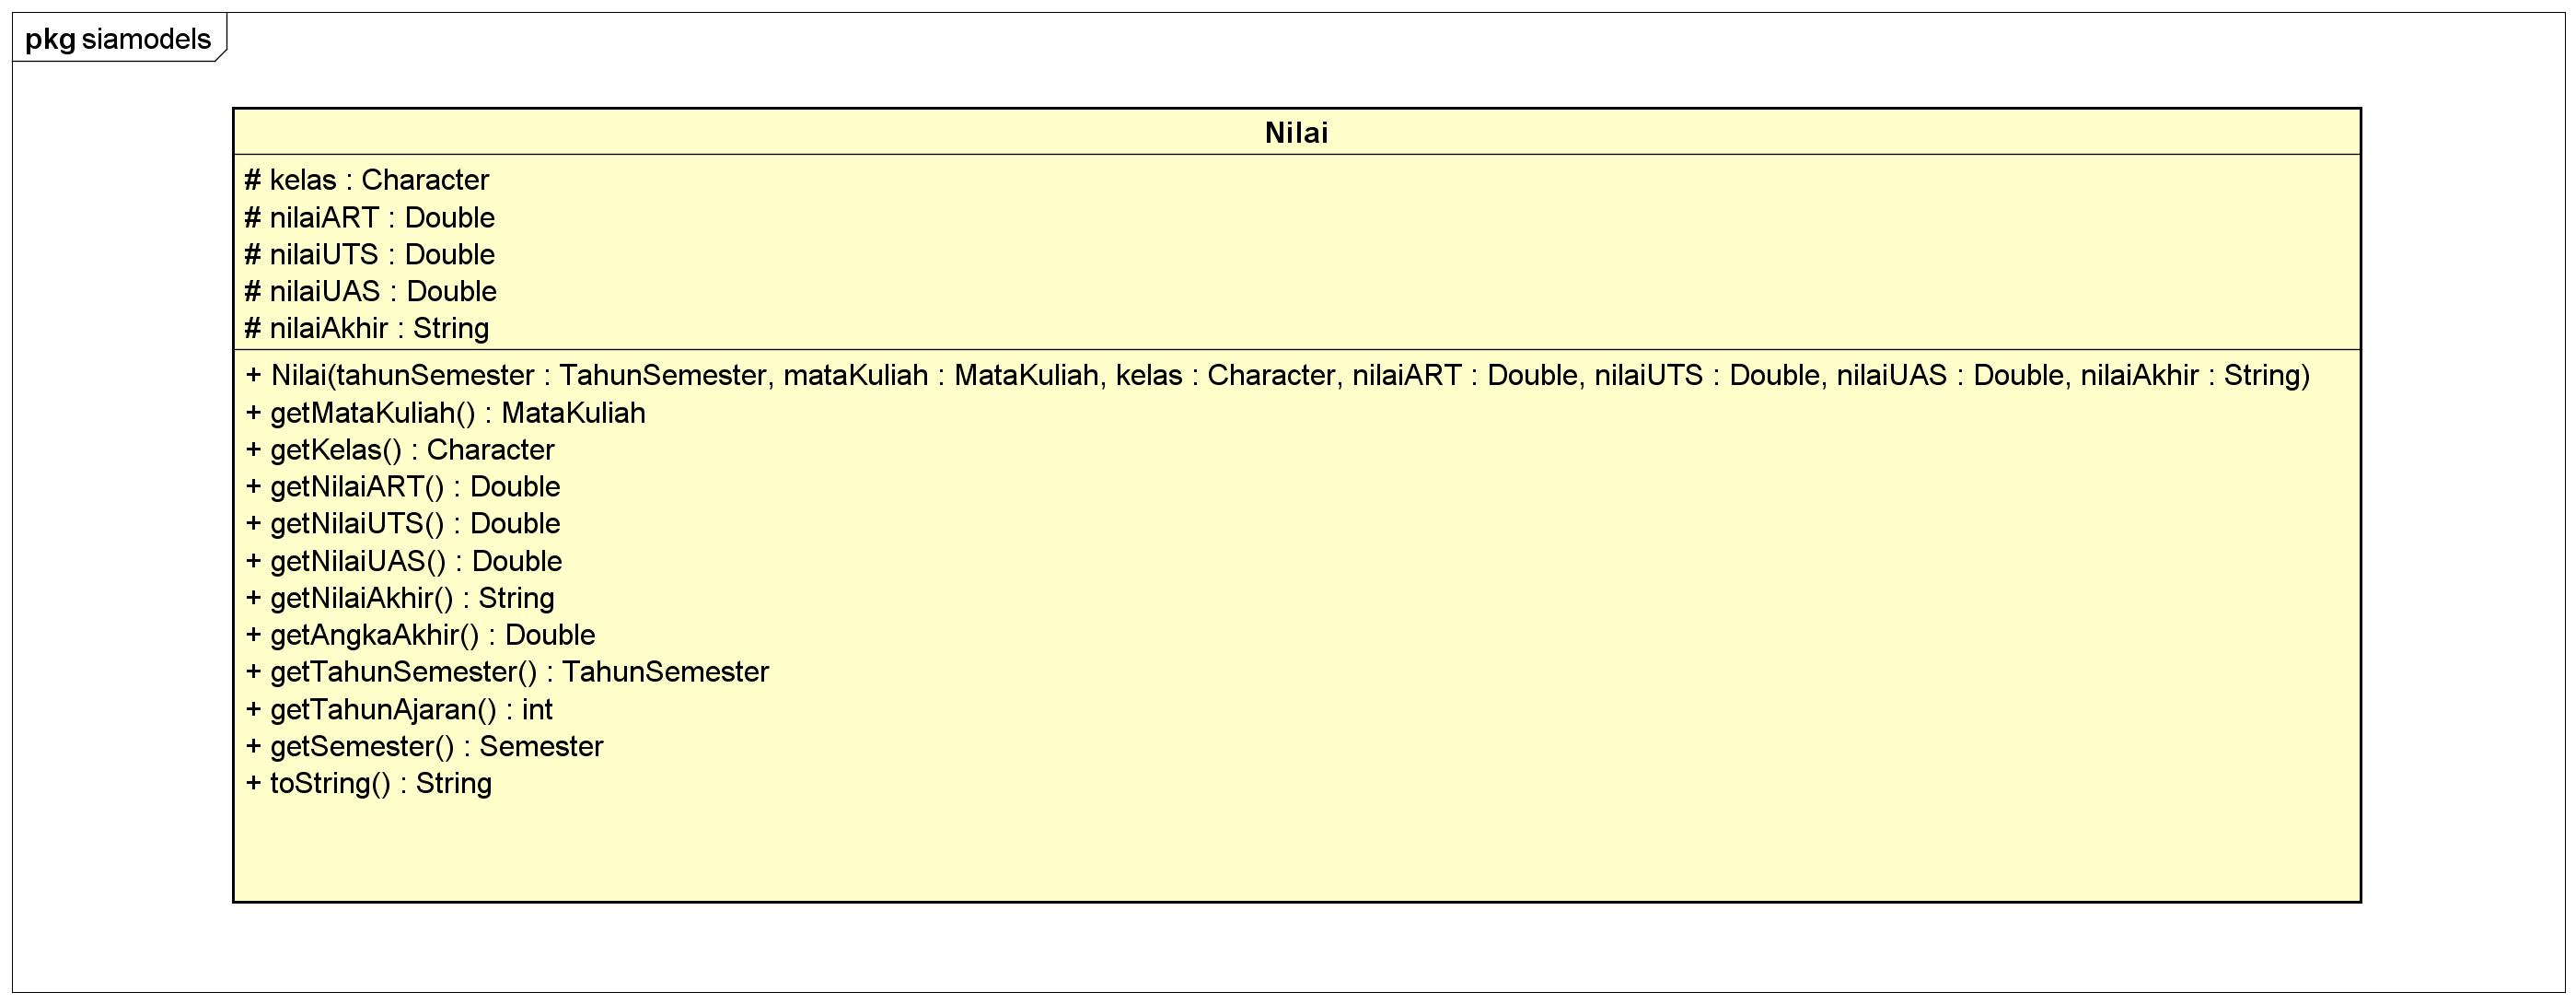
\includegraphics[scale=0.15]{Gambar/class-diagram-siamodels-new}
		\caption{Diagram Kelas SIAModels Bagian \texttt{Nilai}}
		\label{fig:siamodels_class_2018}
		\end{figure}

		\begin{figure}[H]
		\centering
		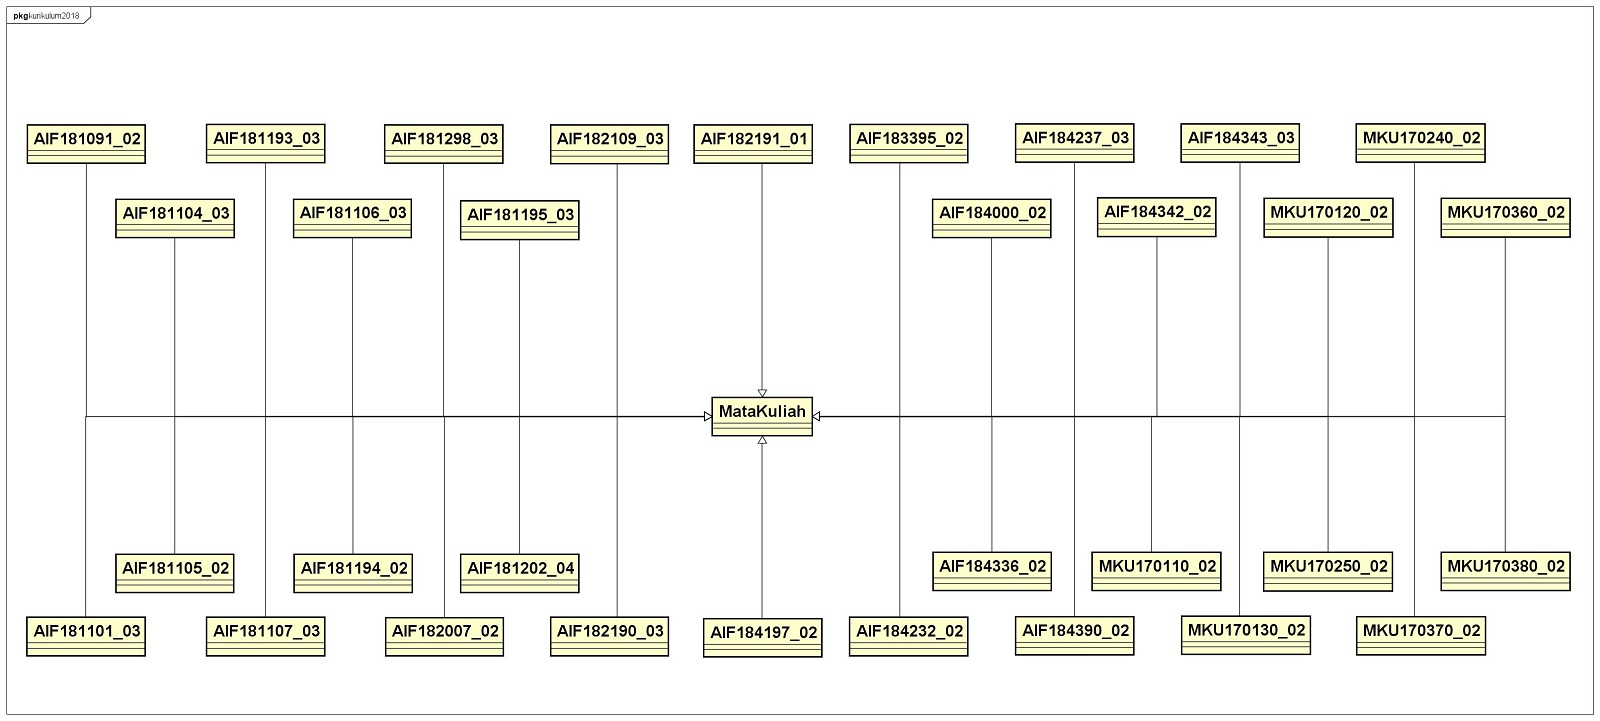
\includegraphics[scale=0.35]{Gambar/class-diagram-siamodels-mk-kurikulum-2018-2}
		\caption{Diagram Kelas SIAModels \textit{Package} \texttt{kurikulum2018} 1}
		\label{fig:siamodels_class_2018_kurikulum_1}
		\end{figure}

		\begin{figure}[H]
		\centering
		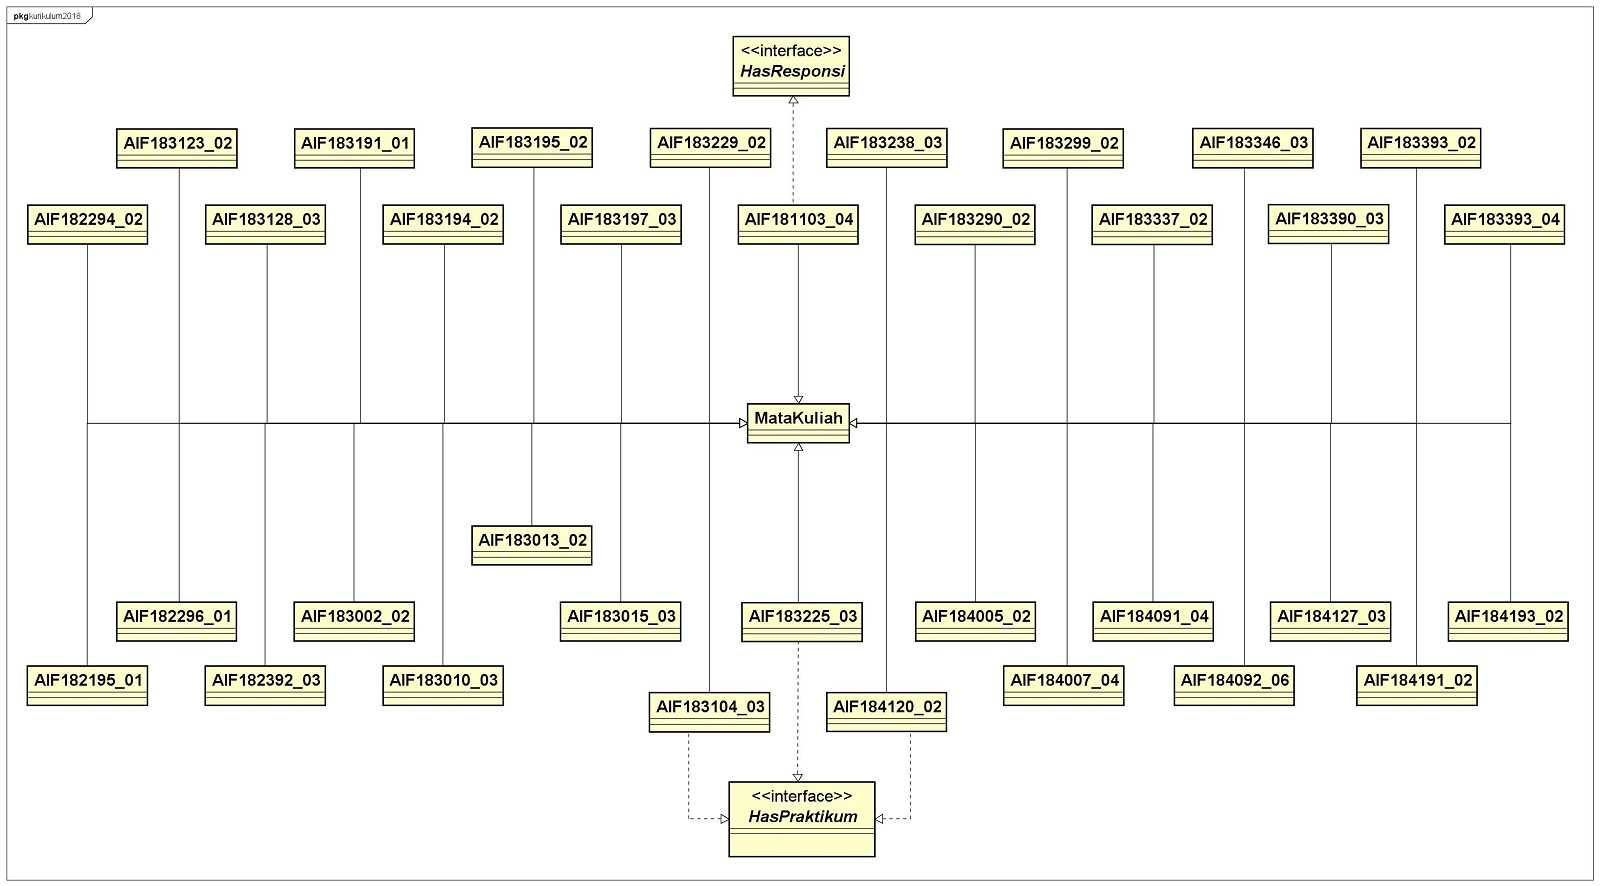
\includegraphics[scale=0.35]{Gambar/class-diagram-siamodels-mk-kurikulum-2018-1}
		\caption{Diagram Kelas SIAModels \textit{Package} \texttt{kurikulum2018} 2}
		\label{fig:siamodels_class_2018_kurikulum_2}
		\end{figure}

		\begin{figure}[H]
		\centering
		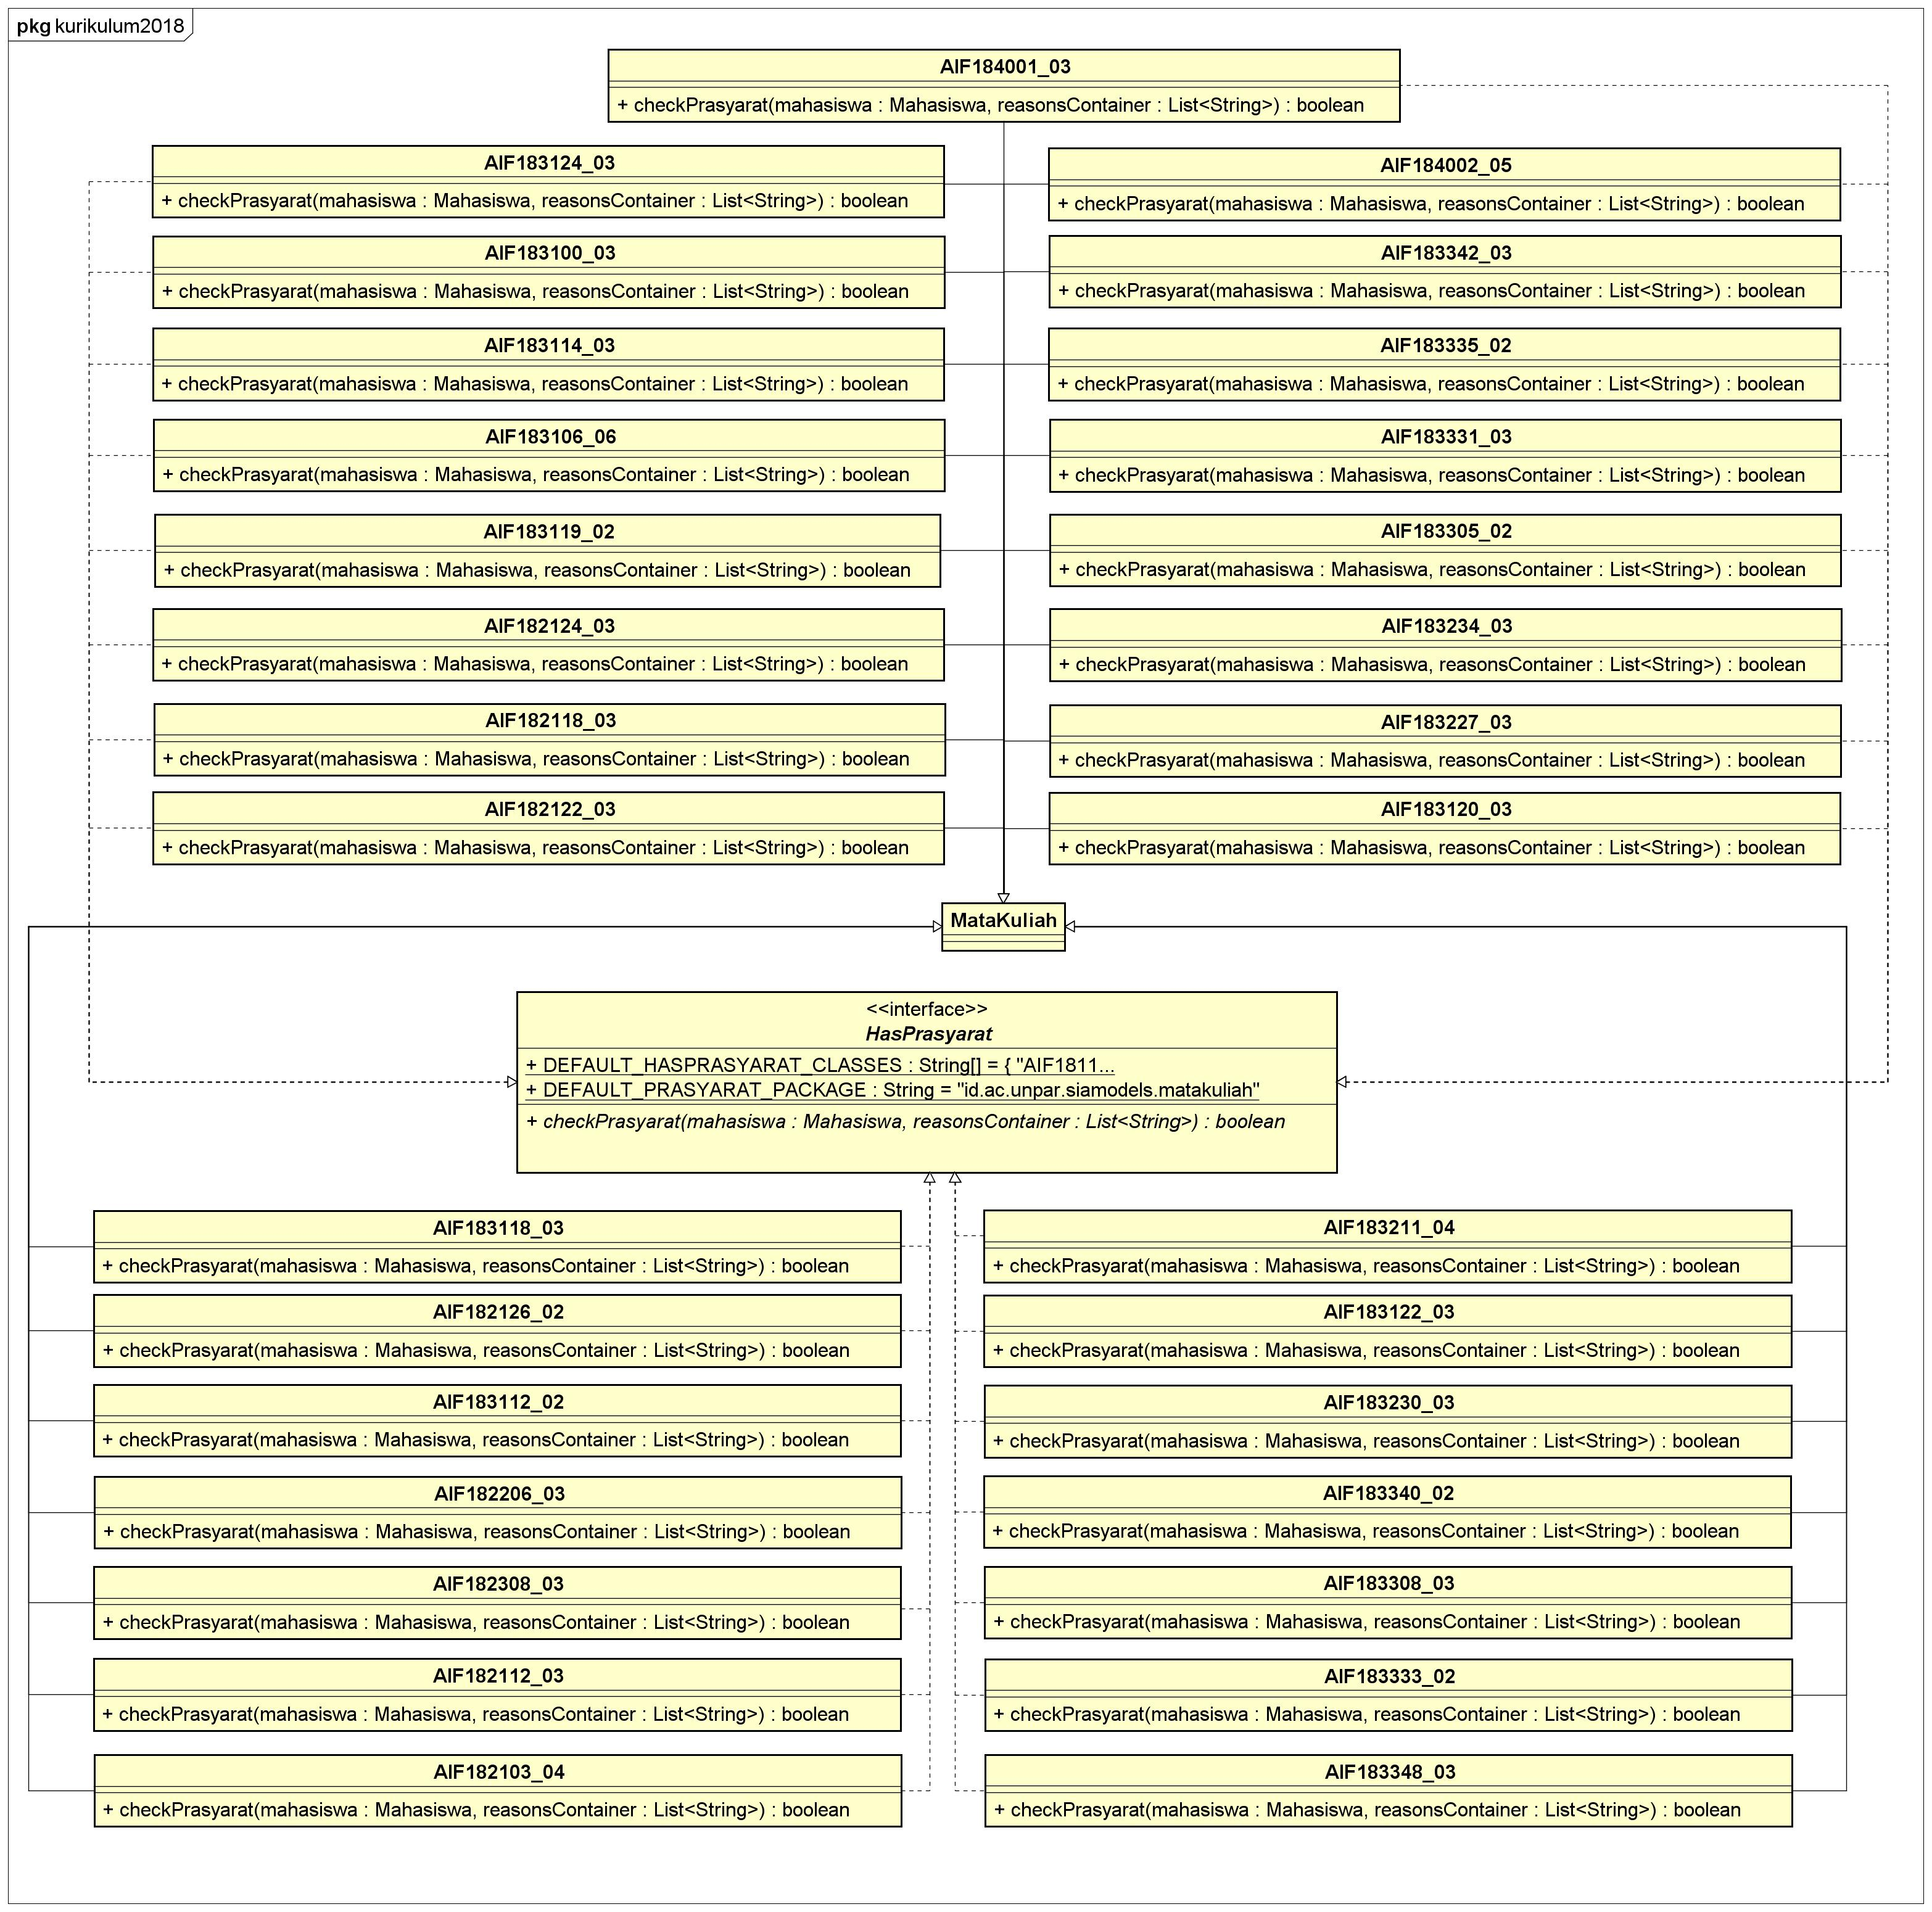
\includegraphics[scale=0.135]{Gambar/class-diagram-siamodels-mk-kurikulum-2018-3}
		\caption{Diagram Kelas SIAModels \textit{Package} \texttt{kurikulum2018} 3}
		\label{fig:siamodels_class_2018_kurikulum_3}
		\end{figure}

		\begin{figure}[H]
		\centering
		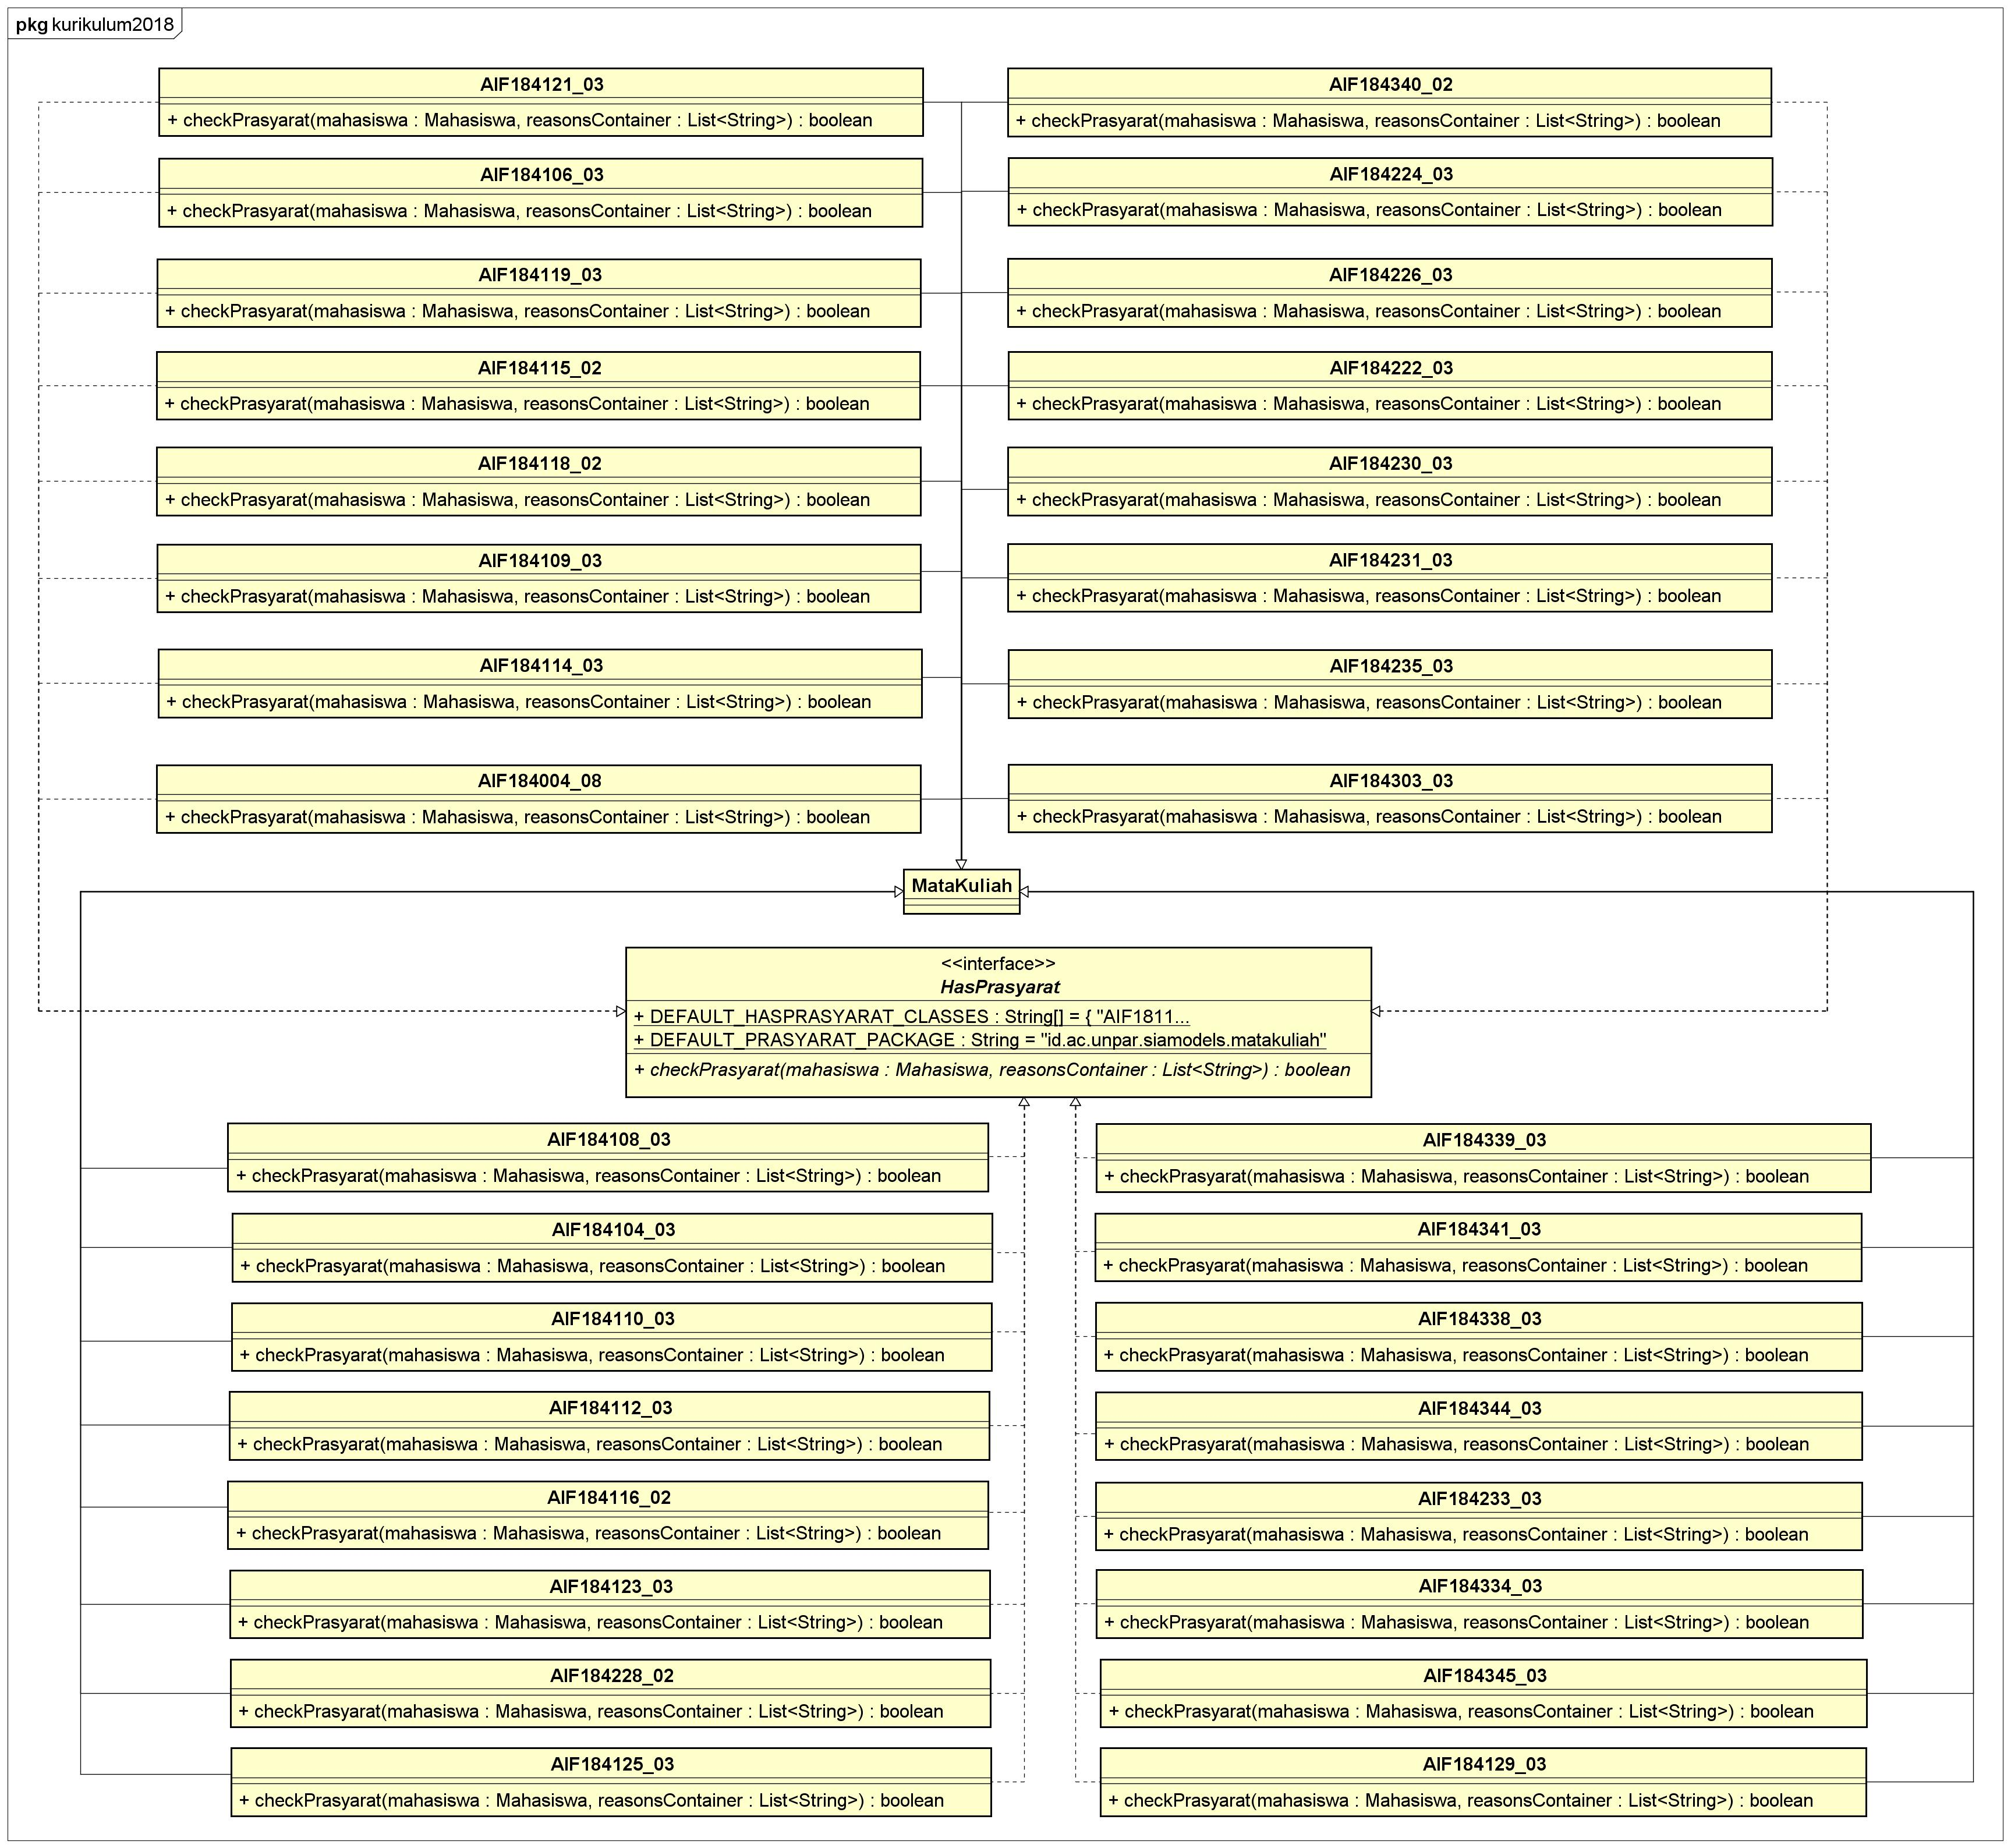
\includegraphics[scale=0.105]{Gambar/class-diagram-siamodels-mk-kurikulum-2018-4}
		\caption{Diagram Kelas SIAModels \textit{Package} \texttt{kurikulum2018} 4}
		\label{fig:siamodels_class_2018_kurikulum_4}
		\end{figure}

		\begin{figure}[H]
		\centering
		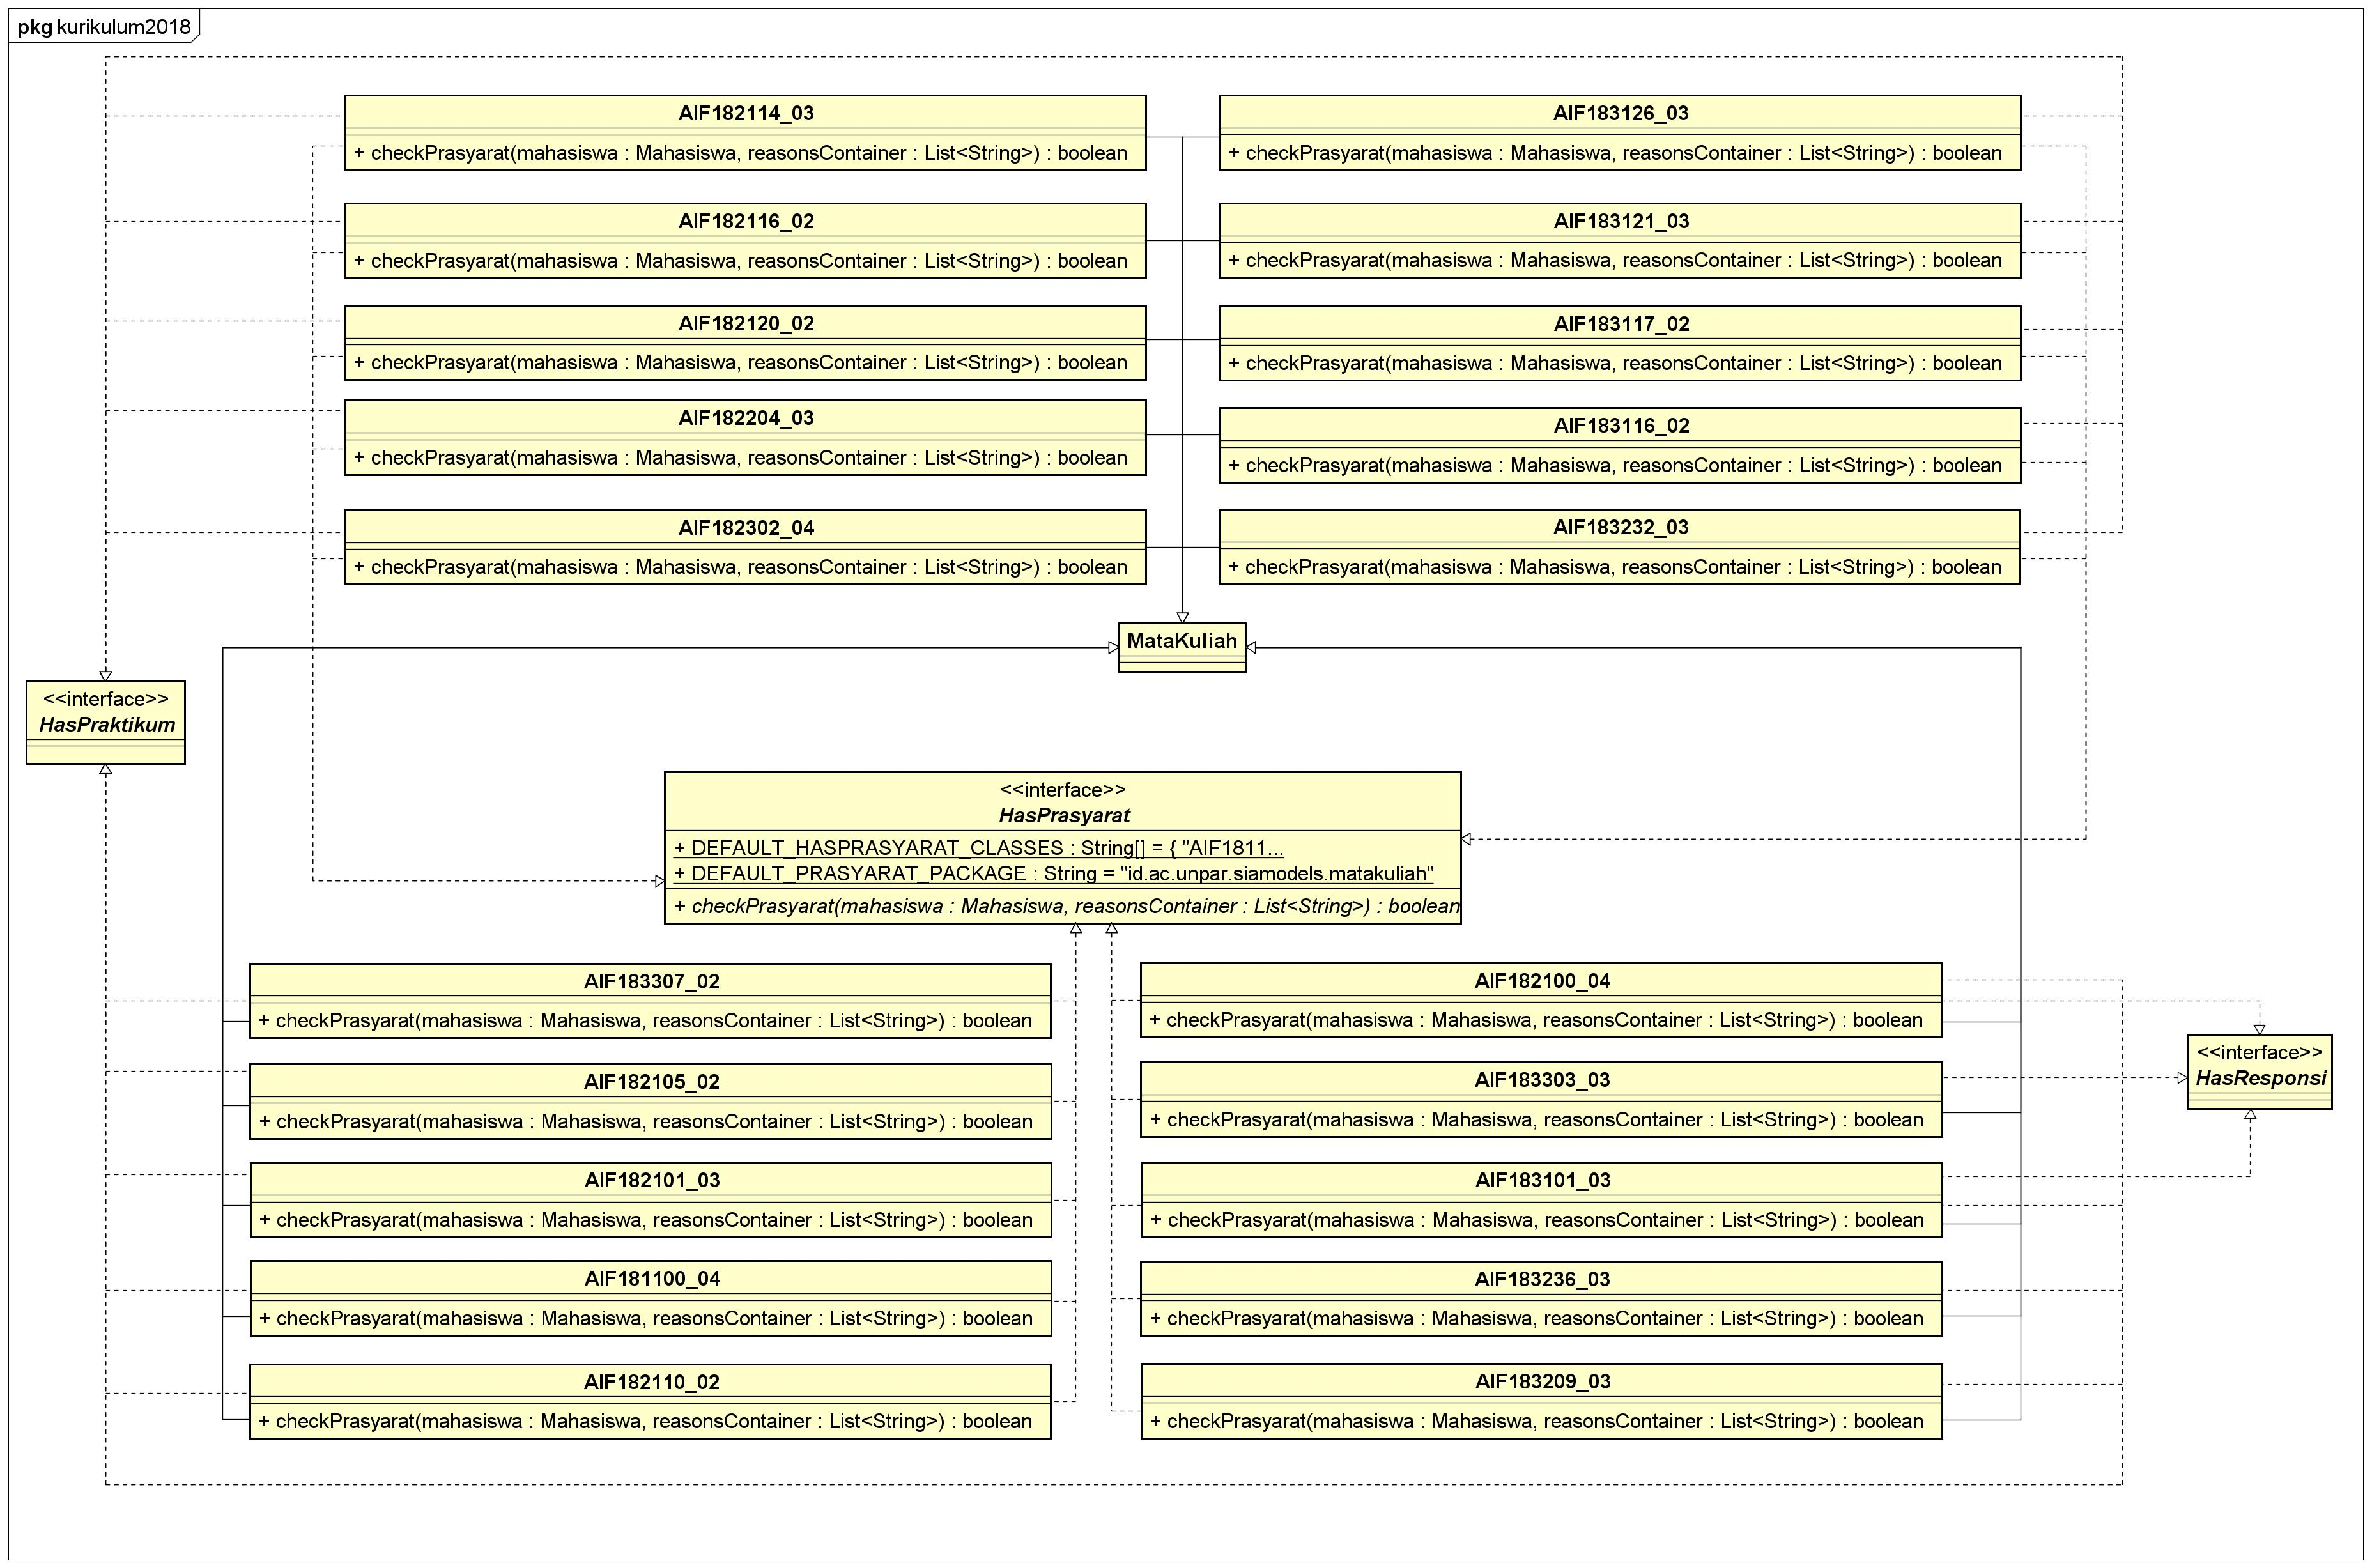
\includegraphics[scale=0.105]{Gambar/class-diagram-siamodels-mk-kurikulum-2018-5}
		\caption{Diagram Kelas SIAModels \textit{Package} \texttt{kurikulum2018} 5}
		\label{fig:siamodels_class_2018_kurikulum_5}
		\end{figure}
		
	\end{enumerate}

\section{Pencapaian Rencana Kerja}
Langkah-langkah kerja yang berhasil diselesaikan dalam Skripsi 1 ini adalah sebagai berikut:
\begin{enumerate}
\item Mempelajari IFStudentPortal dan SIAModels saat ini
\item Melakukan Studi Literatur mengenai Kurikulum 2018 dan Skripsi Herfan Heryandi.
\item Mengimplementasikan sebagaian kurikulum 2018 untuk SIAModels
\item Menganalisis IFStudentPortal dan SIAModels akibat kurikulum 2018
\item Melakukan Perancangan diagram kelas untuk perubahan akibat kurikulum 2018
\item Menulis sebagian dokumen skripsi yaitu bab 1, bab 2, bab 3, dan 4(subbab 4.1)
\end{enumerate}

\vspace{1cm}
\centering Bandung, \tanggal\\
\vspace{2cm} \nama \\ 
\vspace{1cm}

Menyetujui, \\
\ifdefstring{\jumpemb}{2}{
\vspace{1.5cm}
\begin{centering} Menyetujui,\\ \end{centering} \vspace{0.75cm}
\begin{minipage}[b]{0.45\linewidth}
% \centering Bandung, \makebox[0.5cm]{\hrulefill}/\makebox[0.5cm]{\hrulefill}/2013 \\
\vspace{2cm} Nama: \pembA \\ Pembimbing Utama
\end{minipage} \hspace{0.5cm}
\begin{minipage}[b]{0.45\linewidth}
% \centering Bandung, \makebox[0.5cm]{\hrulefill}/\makebox[0.5cm]{\hrulefill}/2013\\
\vspace{2cm} Nama: \pemB \\ Pembimbing Pendamping
\end{minipage}
\vspace{0.5cm}
}{
% \centering Bandung, \makebox[0.5cm]{\hrulefill}/\makebox[0.5cm]{\hrulefill}/2013\\
\vspace{2cm} Nama: \pembA \\ Pembimbing Tunggal
}
\end{document}

